% !TEX encoding = UTF-8 Unicode

\documentclass[esurf, manuscript]{copernicus}

% packages
\usepackage{tabu}
\usepackage{booktabs}
\usepackage{graphicx}
\usepackage[export]{adjustbox}
\usepackage[utf8]{inputenc}
\usepackage{listings}

\begin{document}

\title{\lowercase{r.sim.terrain}: a dynamic landscape evolution model} % in open source GIS

\Author[1,2]{Brendan Alexander}{Harmon}
\Author[1,3]{Helena}{Mitasova}
\Author[1,3]{Anna}{Petrasova}
\Author[1,3]{Vaclav}{Petras}

\affil[1]{Center for Geospatial Analytics, North Carolina State University, Raleigh, North Carolina, United States of America}
\affil[2]{Robert Reich School of Landscape Architecture, Louisiana State University, Baton Rouge, Louisiana}
\affil[3]{Department of Marine, Earth, and Atmospheric Sciences, North Carolina State University, Raleigh, North Carolina, United States of America}

\runningtitle{\lowercase{r.sim.terrain}: a dynamic landscape evolution model}

\runningauthor{Brendan Harmon}

\correspondence{Brendan Harmon (brendan.harmon@gmail.com)}

\received{}
\pubdiscuss{} %% only important for two-stage journals
\revised{}
\accepted{}
\published{}

\firstpage{1}

\maketitle

\begin{abstract}
While there are numerical landscape evolution models
that simulate how steady state flows of water and sediment
reshape topography over long periods of time, 
this is the first to simulate short-term topographic change 
for both steady state and dynamic flow regimes. 
It is a process-based, spatially distributed model
that uses the water and sediment flow continuity equations
to simulate how overland sediment mass flows 
reshape topography. 
This either steady state or dynamic model can simulate 
how topography will evolve for a range of hydrologic soil erosion regimes
based on topographic, land cover, soil, and rainfall parameters. 
A case study demonstrates how the behavior and results of 
the dynamic model differ the steady state model. 
The dynamic model is more accurate and 
demonstrates cross-scale interactions between 
topographic form and sediment flow processes.
\end{abstract}

\copyrightstatement{...}

\introduction  %% \introduction[modified heading if necessary]
Landscape evolution models represent how the surface of the earth changes over time. 
Most studies of landscape evolution have been descriptive, 
but a number of numerical landscape evolution models 
have been developed that simulate elevational change over time 
\citep{Temme2013}. 
% numerical models
Numerical landscape evolution models
such as the Channel-Hillslope Integrated Landscape Development (CHILD) model 
\citep{Tucker2001} 
and SIBERIA \citep{Willgoose2005}
simulate steady state flows over long temporal scales. 
% recent development
Landlab,
\footnote{\url{http://landlab.github.io/}}
a new Python library for numerically modeling Earth surface processes
\citep{Hobley2017},
has components for simulating landscape evolution such as the 
Stream Power with Alluvium Conservation and Entrainment (SPACE) 
model \citep{Shobe2017}.
% research questions
There are still, however, major research questions 
to address in the theoretical foundations of erosion modeling 
such as how erosional processes scale over time and space 
and how sediment detachment and transport interact \citep{Mitasova2013}. 
% dynamic evolution
A dynamic landscape evolution model is needed to study
fine-scale spatial and short-term temporal erosional processes
such as gully formation and the development of microtopography. 
While most numerical landscape evolution models 
simulate peak flows at steady state
(see Table~\ref{table:evolution_models}),
short-term erosional processes like gully formation can be dynamic
with significant morphological changes happening within minutes
before flows reach steady state. 

% steady state versus dynamic
At the beginning of a rainfall event 
the overland water flow regime is dynamic -- 
its depth changes at a variable rate over time and space. 
If the intensity of rainfall continues to change throughout the event
then the flow regime will remain dynamic. 
% steady state
If, however, the overland flow reaches a peak rate
then the hydrologic regime is considered to be at steady state.
At steady state:
% steady state eq.
\begin{equation}
\label{eq:steady_state}
{\partial h(x,y,t) \over \partial t} = 0 %frac
\end{equation}
%
{\small
\noindent
where: \\
\noindent
\hspace*{0.5em} $(x,y)$ is the position ($m$)\\
\hspace*{0.5em} $t$ is the time ($s$) \\
\hspace*{0.5em} $h(x,y,t)$ is the depth of overland flow ($m$)\\
}

% gully formation
Gullies are eroded, steep banked channels 
formed by ephemeral, concentrated flows of water.
A gully forms when overland waterflow
converges in a knickzone
-- a concave space with steeper slopes than its surroundings -- 
during intense rainfall events.  
When the force of the water flow concentrated in the knickzone
is enough to detach and transport large amounts of sediment,
an incision begins to form at the apex of the knickzone 
-- the knickpoint or headwall.
As erosion continues the knickpoint begins to migrate upslope
and the nascent gully channel widens,
forming steep channel banks. 
Multiple incisions initiated by different knickpoints 
may merge into a gully channel
and multiple channels may merge into a branching gully system. 
This erosive process is dynamic; 
the morphological changes drive further changes 
in a positive feedback loop
until water flow reaches steady state. 
When the gully initially forms 
the soil erosion regime should be detachment capacity limited
with the concentrated flow of water in the channel of the gully 
detaching large amounts of sediment and transporting it to the foot of the gully, 
potentially forming a depositional fan. 
After the initial formation of the gully
the soil erosion regime may change.
If the intensity of the rainfall decreases
the regime may switch to erosion-deposition. 
Subsequent rainfall events may trigger further 
knickpoint formation and upslope migration, channel incision and widening, and
depositional fan and ridge formation. 
Between high intensity rainfall events, 
lower intensity events and gravitational diffusion
may gradually smooth the shape of the gully. 
Eventually, if detachment capacity significantly exceeds transport capacity, 
the gully may fill with sediment. 

% gully monitoring
Gully erosion rates and evolution
can be monitored in the field 
or modeled on the computer. 
% field methods
Field methods include
dendrogeomorphology \citep{Malik2008} and 
permanent monitoring stakes for recording erosion rates, 
extensometers for recording mass wasting events, 
weirs for recording water and suspended sediment discharge rates, 
and time series of surveys using 
total station theodolites \citep{Thomas2004},
unmanned aerial systems (UAS),
airborne lidar, and terrestrial lidar \citep{Starek2011,Bechet2016}.

% high resolution topographic data
With terrestrial lidar, airborne lidar and 
UAS photogrammetry
there is now high enough resolution topographic data 
to morphometrically analyze and 
numerically model fine-scale landscape evolution in GIS
including processes such as gully formation 
and the development of microtopography. 
% gully simulation
Gully erosion has been simulated with 
the Revised Universal Soil Loss Equation Version 2 (RUSLER)
in conjunction with the Ephemeral Gully Erosion Estimator (EphGEE)
\citep{Dabney2014},
while gully evolution
has been simulation for detachment capacity limited erosion regimes
with the Simulation of Water Erosion (SIMWE) model
\citep{Koco2011, Mitasova2013}. 
% what is needed?
Now numerical landscape evolution models 
that can simulate 
steady state and dynamic flow regimes
and can dynamically switch between soil erosion regimes 
are needed to study 
fine-scale spatial and short-term temporal erosional processes.

% aim
The numerical landscape evolution model 
\lowercase{r.sim.terrain} was developed to 
simulate the spatiotemporal evolution of landforms
caused by shallow overland water and sediment flows
at spatial scales ranging from
square meters to thousands of kilometers
and temporal scales ranging from minutes to years. 
% objectives
This open source, GIS-based landscape evolution model can
simulate either steady state or dynamic flow regimes, 
dynamically switch between soil erosion regimes, and
simulate the evolution of fine-scale morphological features 
such as ephemeral gullies.
% questions
It was designed as a research tool for
studying how erosional processes scale over time and space,
comparing empirical and process-based models, 
comparing steady state and dynamic flow regimes, and
studying the role of dynamic flow regimes in fine-scale morphological change. 
% testing
\lowercase{r.sim.terrain} was tested with a regional scale ($650 \unit{km}^{2}$) case study
and a subwatershed scale ($450 \unit{m}^{2}$) case study. 
At the subwatershed scale simulations were compared against 
a time-series of lidar surveys.
% novelty

\section{r.sim.terrain}
\lowercase{r.sim.terrain}
is a process-based, spatially distributed landscape evolution model
that simulates topographic changes
caused by shallow, overland water flow
across a range of spatiotemporal scales and soil erosion regimes
using either
the Simulated Water Erosion (SIMWE) model, 
the 3-Dimensional Revised Universal Soil Loss Equation (RUSLE 3D) model,
or the Unit Stream Power Erosion Deposition (USPED) model.  
% simwe
SIMWE is a physics-based simulation
that uses a Monte Carlo path sampling method
to solve the water and sediment flow equations 
for detachment limited, transport limited, and erosion-deposition 
soil erosion regimes \citep{Mitasova2004}. 
With SIMWE 
\lowercase{r.sim.terrain}
uses the modeled flow of sediment 
-- a function of water flow and soil detachment and transport parameters -- 
to estimate the net erosion and deposition rates. 
% rusle3d
RUSLE3D is an empirical equation for sediment flows 
in detachment capacity limited soil erosion regimes \citep{Mitasova1996}. 
With RUSLE3D
\lowercase{r.sim.terrain}
uses an event-based erosivity factor, 
the slope, the flow accumulation, and a 3D topographic factor
to model sediment flow. 
% usped
USPED is an empirical equation for net erosion and deposition 
in transport capacity limited soil erosion regimes. 
With USPED 
\lowercase{r.sim.terrain}
uses an event-based erosivity factor, 
the slope and aspect, the flow accumulation, and a 3D topographic factor
to model erosion-deposition as the
the divergence of sediment flows. 
% evolution
For each of the models 
topographic change is derived at each time step
from the sediment flow or net erosion-deposition rate
and gravitational diffusion.
% regimes
\lowercase{r.sim.terrain} 
can simulate steady state or dynamic flow regimes.
During simulations with SIMWE 
\lowercase{r.sim.terrain}
can switch between 
detachment limited, transport limited, and erosion-deposition 
soil erosion regimes.

% capabilities
\lowercase{r.sim.terrain}
can simulate the evolution of gullies
including processes such as 
knickpoint migration,
channel incision, 
channel widening, and
scour pool and depositional riffle formation
along the thalweg of the gully. 
% applications
Applications include 
geomorphological research,
erosion control, 
landscape restoration, 
and scenario development 
for landscape planning and management.
% scale
r.sim.terrain can simulate landscape evolution 
over a wide range of spatial scales from small watersheds 
less than ten square kilometers
with SIMWE
to regional watersheds
of thousands of square kilometers
with USPED or RULSE3D. 

% implementation
This model has been implemented 
as a Python add-on module 
for the free, open source
Geographic Resources Analysis Support System (GRASS) GIS
\footnote{\url{https://grass.osgeo.org/}}. 
The source code is available at 
\url{https://github.com/baharmon/landscape\_evolution} 
under the GNU General Public License v2. % cite software release doi
%
This highly adaptable
geographic information system (GIS)-based implementation
was developed as a research tool for studying 
the interaction of sediment detachment and transport
and the scaling of erosional processes over time and space. % <--- revise
% parallel processing
It supports multithreading and parallel processing
to efficiently compute simulations 
using large, high resolution topographic datasets.
%
The landscape evolution model 
can be installed in GRASS GIS as an add-on module 
with the command: 
\begin{lstlisting}
g.extension r.sim.terrain url=github.com/baharmon/landscape_evolution
\end{lstlisting}

	% see landlab paper and others on implementation and dev

% design principles
	% features 
		% in table
		% multiprocessing / parallel processing, dynamics, scales, models, etc

%\subsection{Conceptual model}
%Diagram\\
%Dynamic vs steady state \\
%Determine mode \\
%Run erosion model \\
%Gravitational diffusion \\

% -------------------------- TABLE OF MODELS -----------------------------

% table of erosion models
\begin{table*}
\small
\caption{GIS-based soil erosion models}
\begin{tabu} to \textwidth {XXXXXl}
\toprule
Model & Spatial scale &  Temporal scale & Representation & Implementation & Reference\\
\midrule
GeoWEPP & watershed & continuous & raster & \href{http://geowepp.geog.buffalo.edu/}{ArcGIS module} & \citep{Flanagan2013}\\
AGWA  & watershed & event -- & vector & \href{https://www.tucson.ars.ag.gov/agwa/}{ArcGIS module} & \citep{Guertin2015}\\
&& continuous\\
RUSLE3D & regional & continuous & raster & map algebra & \citep{Mitasova1996}\\
USPED & watershed & continuous & raster & map algebra & \citep{Mitasova1996}\\
SIMWE & watershed & event -- & raster & \href{https://grass.osgeo.org/grass74/manuals/r.sim.sediment.html}{GRASS modules} & \citep{Mitas1998}\\
&& continuous\\
\bottomrule
\\
%\multicolumn{6}{c}{Adapted from Mitasova et al. \citep{Mitasova2013}}
\end{tabu}
\label{table:erosion_models} 
\end{table*}

% table of landscape evolution models
\begin{table*}
\small
\caption{Numerical landscape evolution models}
\begin{tabu} to \textwidth {XXXXXll}
\toprule
Model & Spatial scale &  Temporal scale & Representation & Dynamics & Implementation & Reference\\
\midrule
% GOLEM
SIBERIA & regional & continuous & raster & steady state & \href{https://csdms.colorado.edu/wiki/Model:SIBERIA}{Fortran prog.} & \citep{Willgoose2005}\\
CHILD & regional & continuous & mesh & steady state & \href{https://csdms.colorado.edu/wiki/Model:CHILD}{C++ program} & \citep{Tucker2001}\\
Landlab & regional & continuous & raster + mesh & steady state & \href{https://github.com/landlab/}{Python library} & \citep{Hobley2017}\\
r.landscape.evol  & regional & continuous & raster &  steady state & \href{https://grass.osgeo.org/grass74/manuals/addons/r.landscape.evol.html}{GRASS module} & \citep{Barton2010}\\
r.sim.terrain & watershed -- & event -- & raster & dynamic -- & \href{https://github.com/baharmon/landscape_evolution}{GRASS module} &\\ % cite software
& regional & continuous && steady state & &\\
\bottomrule
\\
%\multicolumn{7}{c}{Adapted from Mitasova et al. \citep{Mitasova2013}}
\end{tabu}
\label{table:evolution_models} 
\end{table*}

% regional --->  >10 km2 watershed  $>10^{2}km$
% watershed --->  < 10 km2 watershed  $<10^{2}km$

% -------------------------- MODEL FIGURE -----------------------------

% model figure
\begin{figure}[H]
\center
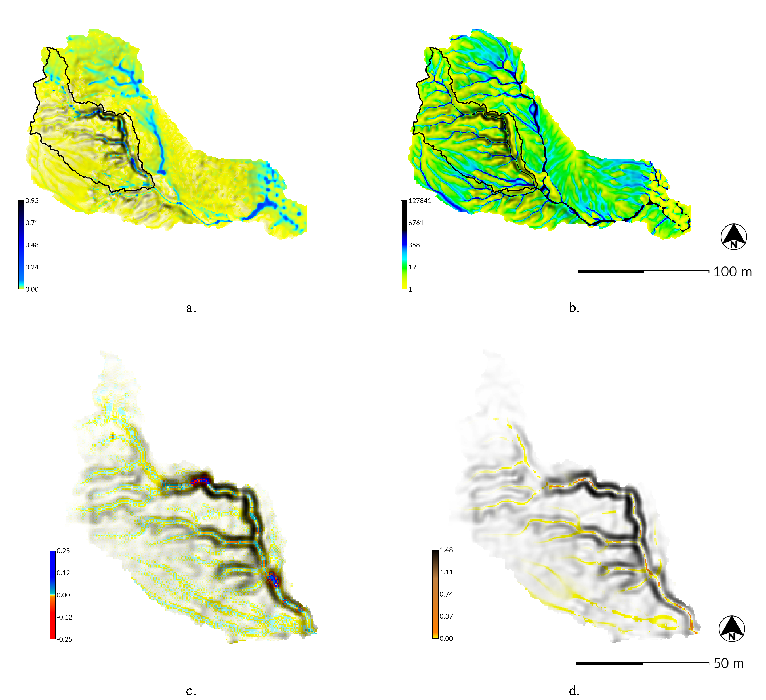
\includegraphics[width=\textwidth,height=0.95\textheight,keepaspectratio]{figures/models.pdf}
\caption{Water and sediment flows simulated by SIMWE 
for a $10~min$ event with $50~mm~hr^{-1}$
and by RUSLE3D with a R-factor of 310
}
\label{fig:models}
\end{figure}

% -------------------------- EROSION-DEPOSITION -----------------------------
\subsection{Simulation of water erosion model} \label{simwe}
% simwe intro
SIMWE -- the Simulation of Water Erosion model -- 
is a physics-based simulation of shallow overland water and sediment flow
that uses a path sampling method to solve the continuity and momentum equations 
with a 2D diffusive wave approximation 
\citep{Mitas1998,Mitasova2001,Mitasova2004}.
% implementation
It has been implemented in GRASS GIS as the modules 
r.sim.water\footnote{\url{https://grass.osgeo.org/grass75/manuals/r.sim.water.html}} 
and r.sim.sediment\footnote{\url{https://grass.osgeo.org/grass75/manuals/r.sim.sediment.html}}.

% overview
In SIMWE mode 
for each time step
\lowercase{r.sim.terrain}
determines the soil erosion regime,
simulates water and sediment flows, 
and then evolves the topography. 
% erdep
In an erosion-deposition regime 
the model 
computes the partial derivatives of the topography,
simulates shallow water flow and erosion-deposition,
and then evolves the topography based on the erosion-deposition rate
and gravitational diffusion.
% transport limited
The same process is used in
a transport capacity limited regime
except that the topography is evolved based on 
the transport limited erosion-deposition rate
and gravitational diffusion.
% detachment  limited
In a detachment capacity limited regime
the model instead
computes the partial derivatives of the topography,
simulates shallow water flow and sediment flow,
and then evolves the topography based on the sediment flow rate
and gravitational diffusion.
% dynamic versus steady state
The model simulates dynamic landscape evolution 
when the time step is less than the travel time 
for a drop of water or a particle of sediment to cross the landscape.
With longer time steps the model simulates steady state dynamics. 

% ------------------------------------------------------------------------------

\subsubsection{Erosion regime}

% Erosion regime
This model can switch erosion regimes at each time step
based on the rainfall intensity $i_r$
and the balance of the sediment detachment capacity $D_c$
and the sediment transport capacity $T_c$
represented by the first order reaction term $\sigma$ 
which depends on soil and landcover properties.
The detachment capacity is the maximum potential 
detachment rate by overland flow, while
the sediment transport capacity 
is the maximum potential sediment flow rate.
When rainfall intensity is very high ($i_r \geq 60 mm~hr^{-1}$)
or $\sigma$ is low ($\sigma \leq 0.01 m^{-1}$),
then the regime is detachment capacity limited. 
%
When rainfall intensity is not very high ($i_r < 60 mm~hr^{-1} $)
and $\sigma$ is high ($\sigma \geq 100 m^{-1}$),
then the regime is transport capacity limited. 
%
When rainfall intensity is not very high 
($i_r<60 mm~hr^{-1}$)
and $\sigma$ is neither high nor low 
($ 0.01 m^{-1}< \sigma < 100 m^{-1}$),
then there is an erosion-deposition regime. \\
% erosion regime eq.
\begin{equation}
\label{eq:regime}
\sigma = {D_c \over T_c}
\end{equation}
{\small
\noindent
where: \\
\noindent
\hspace*{0.5em} $\sigma$  is a first order reaction term ($m^{-1}$)\\
\hspace*{0.5em} $D_c$ is the sediment detachment capacity ($kg~m^{-1}s^{-1}$)\\
\hspace*{0.5em} $T_c$ is the sediment transport capacity ($kg~m^{-1}s^{-1}$)\\
}

% ------------------------------------------------------------------------------

\subsubsection{Shallow water flow}

% Shallow water flow
The SIMWE model
simulates shallow overland water flow
controlled by spatially variable topographic, soil, landcover, and rainfall parameters
by solving the continuity and momentum equations 
for steady state water flow with a path sampling method
(Fig.~\ref{fig:models}a). %(Fig.~\ref{fig:depth}). 
Shallow water flow $q(x,y,t)$ can be approximated by
the bivariate form of the St.~Venant equation:
% shallow water flow eq.
\begin{equation}
\label{eq:water}
{\partial h(x,y,t) \over \partial t} =
 i_e(x,y,t) - \nabla ~ q(x,y,t)
\end{equation}
{\small
\noindent
where: \\
\noindent
\hspace*{0.5em} $(x,y)$ is the position ($m$)\\
\hspace*{0.5em} $t$ is the time ($s$) \\
\hspace*{0.5em} $h(x,y,t)$ is the depth of overland flow ($m$)\\
\hspace*{0.5em} $i_e(x,y,t)$ is the rainfall excess ($m~s^{-1}$) \\
\hspace*{0.5em} (i.e.~rainfall intensity $-$ infiltration $-$ vegetation intercept)\\
\hspace*{0.5em} $\nabla$ is the divergence of the flow vector field\\
\hspace*{0.5em} $q(x,y,t)$ is the water flow per unit width ($m^2~s^{-1}$). \\
}

Diffusive wave effects can be approximated
so that water can flow through depressions 
by integrating a diffusion term $ \propto \nabla^2 [h^{5/3}(x,y)]$ 
into the solution of the continuity and momentum equations 
for steady state water flow.
This equation is solved using a 
Green's function Monte Carlo path sampling method. 
%  diffuse wave eq.
\begin{equation}
\label{eq:difwater}
-{\varepsilon(x,y)\over 2 }\nabla^2 [h^{5/3}(x,y)]
+\nabla ~ [ h(x,y)~v(x,y)] = i_e(x,y)
\end{equation}
{\small
\noindent
 where: \\
 \noindent
 \hspace*{0.5em} $\varepsilon(x,y)$ is a spatially variable diffusion coefficient. \\
}

%% water flow figure
%\begin{figure}[H]
%\center
%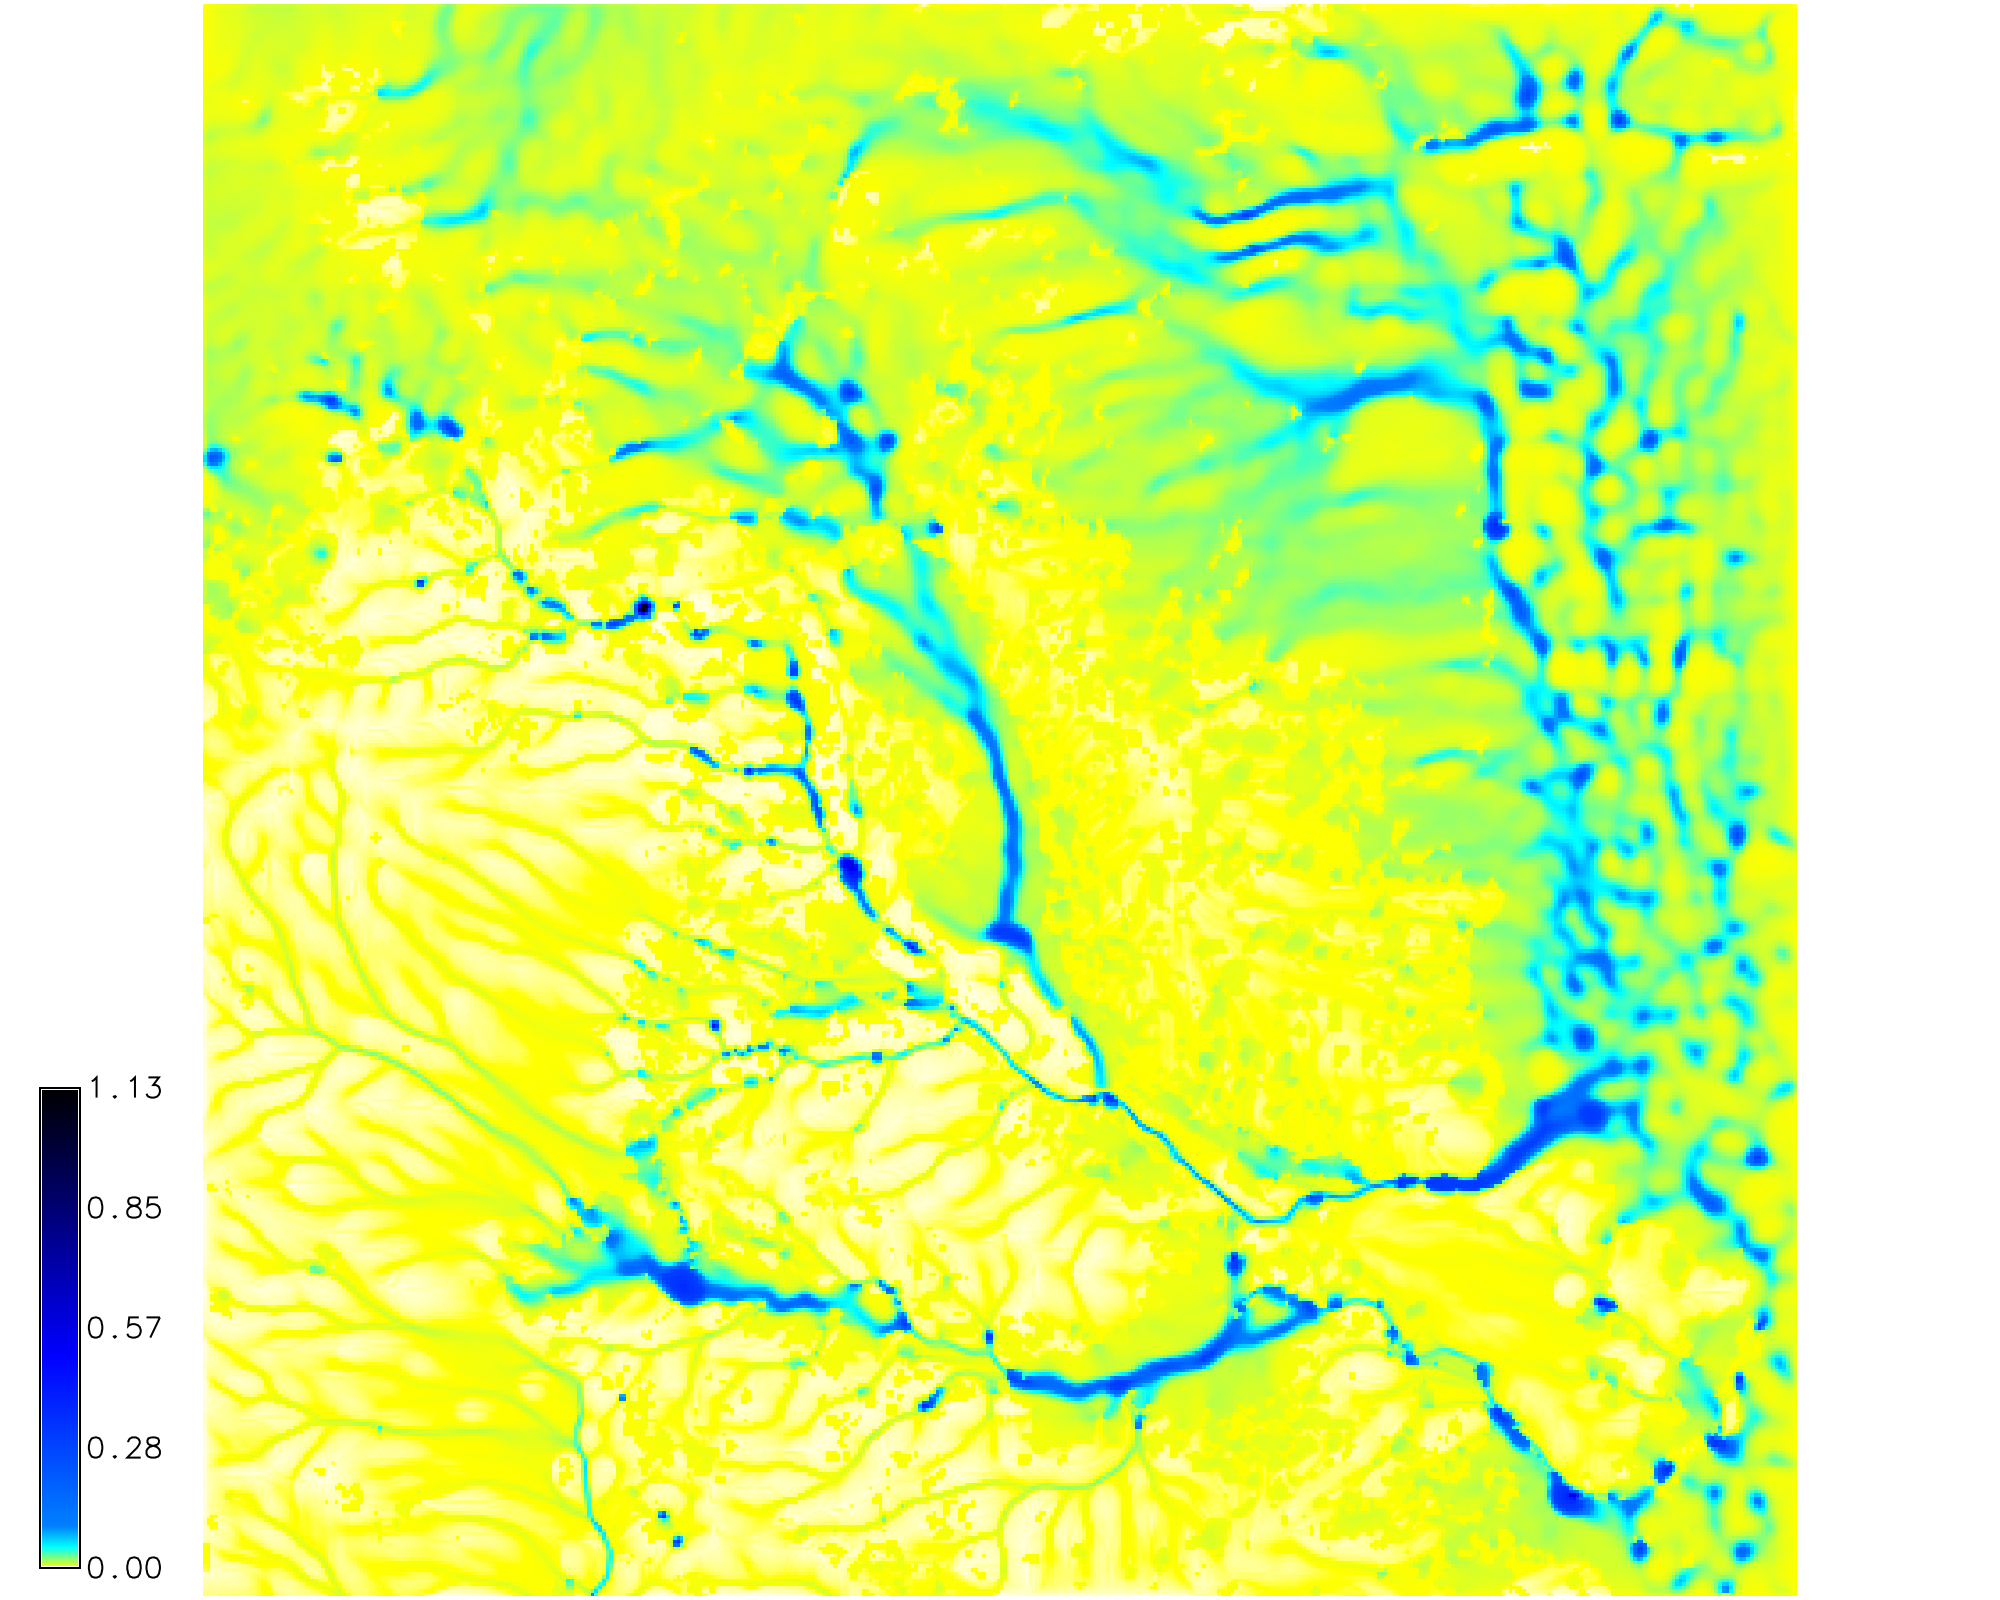
\includegraphics[width=0.75\textwidth]{../images/sample_data/depth_2016.png}
%\caption{Shallow overland water depth $(m)$ simulated by SIMWE  for a $10 min$ event with $50~mm~hr^{-1}$}
%\label{fig:depth}
%\end{figure}

% ------------------------------------------------------------------------------

\subsubsection{Sediment flow}

% Sediment flow
In SIMWE the sediment flow rate $q_s(x,y,t)$ is estimated 
as a function of water flow and sediment concentration
(Fig.~\ref{fig:models}b): %(Fig.~\ref{fig:flux}):
%sediment flow equation
\begin{equation}\label{eq:sedflow} 
q_s(x,y,t) = \rho_s(x,y,t) ~ q(x,y,t)
\end{equation}
{\small
\noindent
where: \\
\hspace*{0.5em} $q_s(x,y,t)$ is the sediment flow rate per unit width ($kg~m^{-1}s^{-1}$)\\
\hspace*{0.5em} $\rho_s(x,y,t)$ is sediment mass density ($kg~m^{-3}$).\\
%\hspace*{0.5em} $q(x,y,t)$ is unit flow discharge vector ($m^{2} s^{-1}$) \\
%\hspace*{0.5em} (i.e.~ the direction and rate of water flow per unit width)\\
}

%% flux figure
%\begin{figure}[H]
%\center
%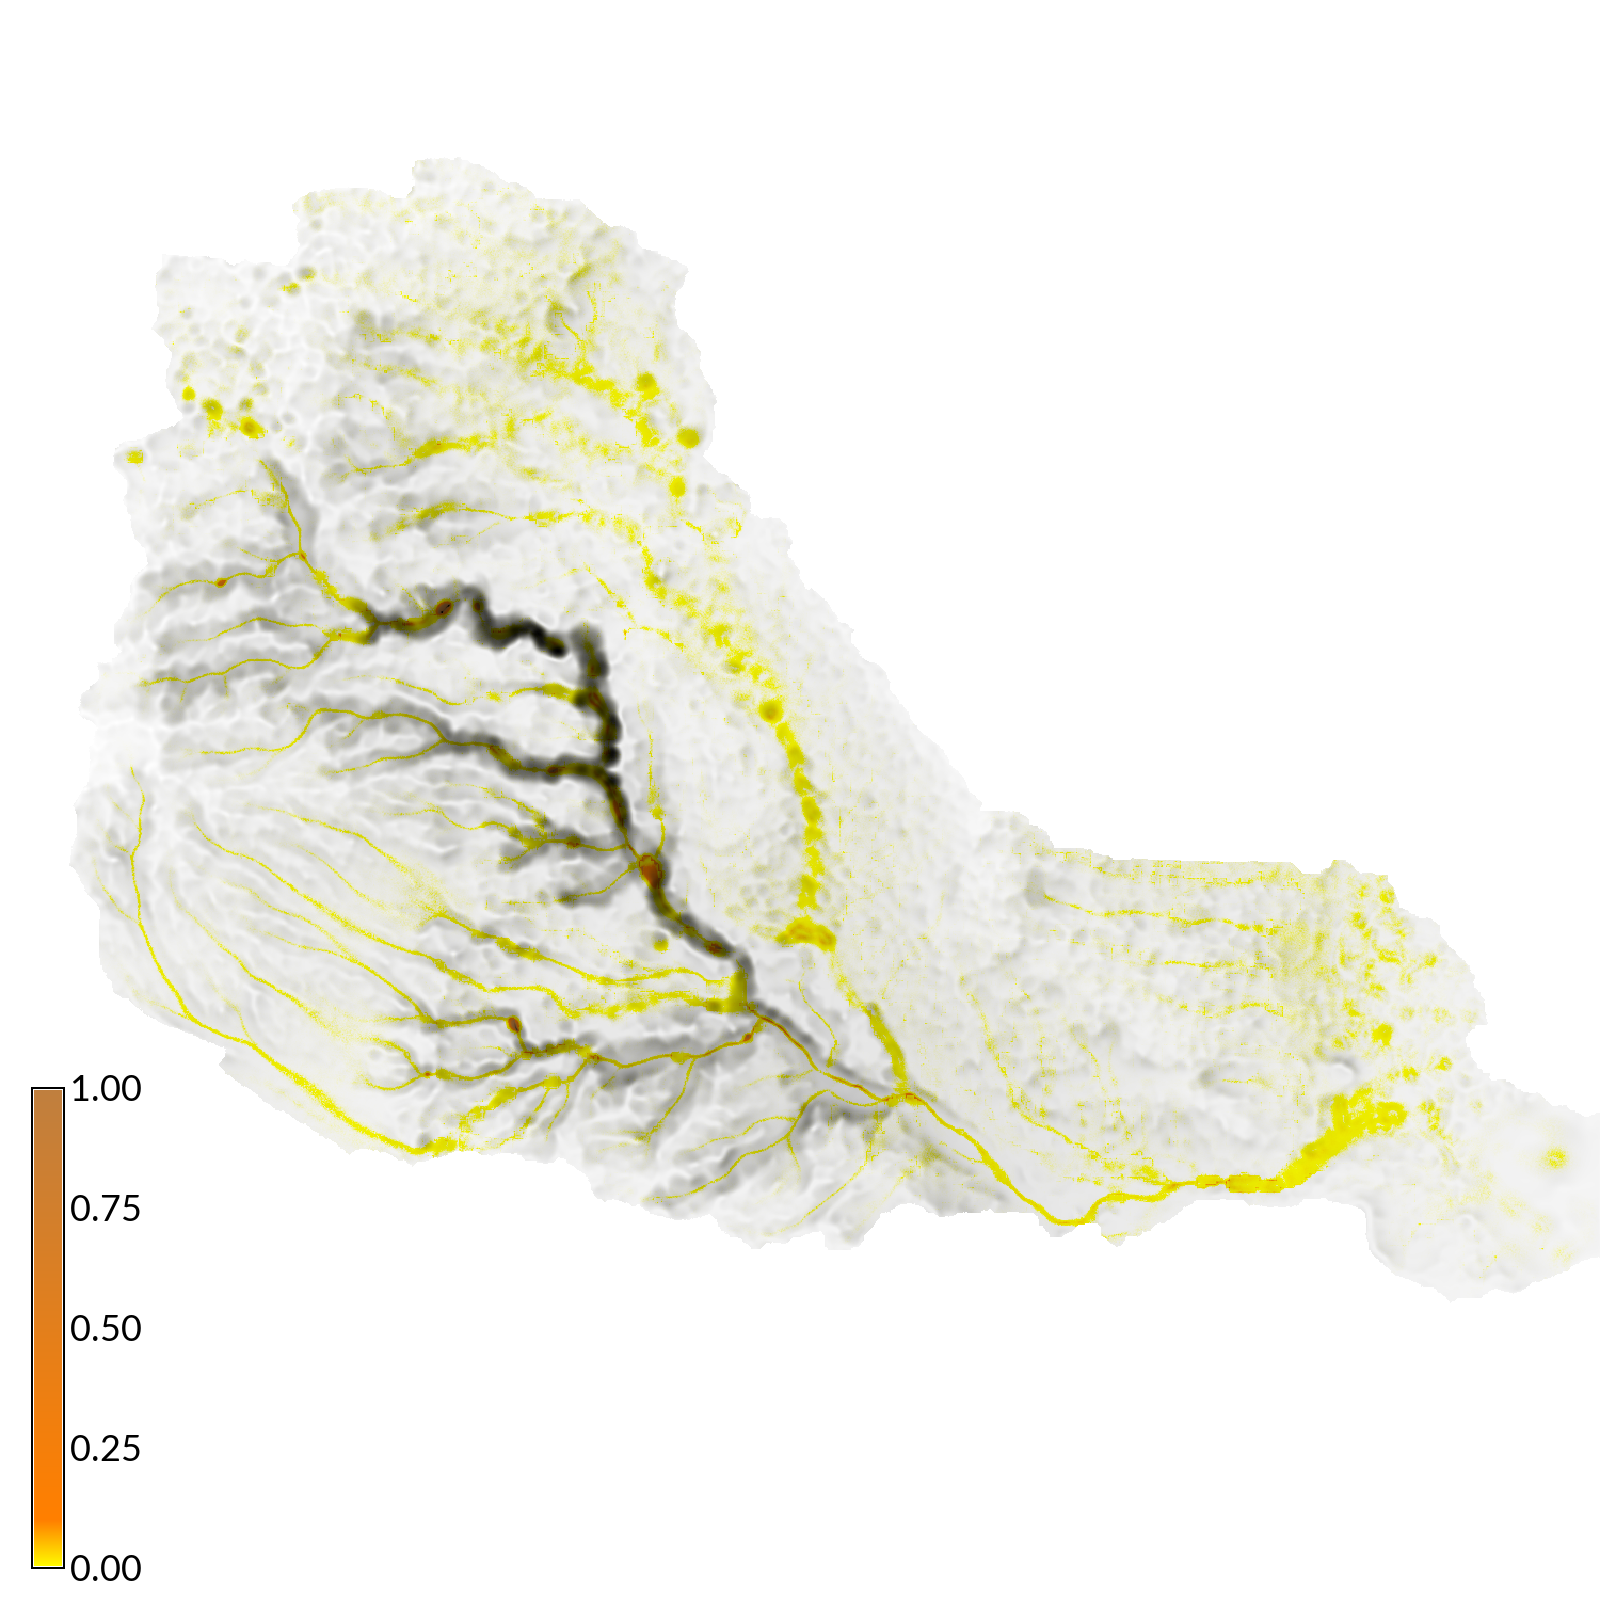
\includegraphics[width=0.75\textwidth]{../images/sample_data/sediment_flux_2016.png}
%\caption{Sediment flux $(kg~m^{-1}~s^{-1})$ simulated by SIMWE}
%\label{fig:flux}
%\end{figure}

% ------------------------------------------------------------------------------

\subsubsection{Erosion-deposition}

% Erosion-deposition
In SIMWE 
the net erosion-deposition rate is estimated
using the bivariate form of sediment continuity equation
to model sediment storage and flow 
based on effective sources and sinks
(Fig.~\ref{fig:models}c). %(Fig.~\ref{fig:erdep}).
Net erosion-deposition $d_s(x,y,t)$
-- the difference between sources and sinks --
is approximated by
the steady state sediment flow equation with diffusion:
% erosion-deposition equation
\begin{equation}\label{eq:sediment} 
d_s(x,y,t) = 
{\partial [\rho_sc(x,y,t)h(x,y,t)] \over \partial t} +
\nabla ~ q_s(x,y,t)
\end{equation}
{\small
\noindent
where: \\
\hspace*{0.5em} $d_s(x,y,t)$ is net erosion-deposition $(kg ~ m^{-2} s^{-1})$.\\
%\hspace*{0.5em} $q_s(x,y,t)$ is the sediment flow rate per unit width ($kg~m^{-1}s^{-1}$)\\
%\hspace*{0.5em} $\rho_s(x,y,t)$ is sediment mass density ($kg~m^{-3}$).\\
}

%% erosion-deposition figure
%\begin{figure}[H]
%\center
%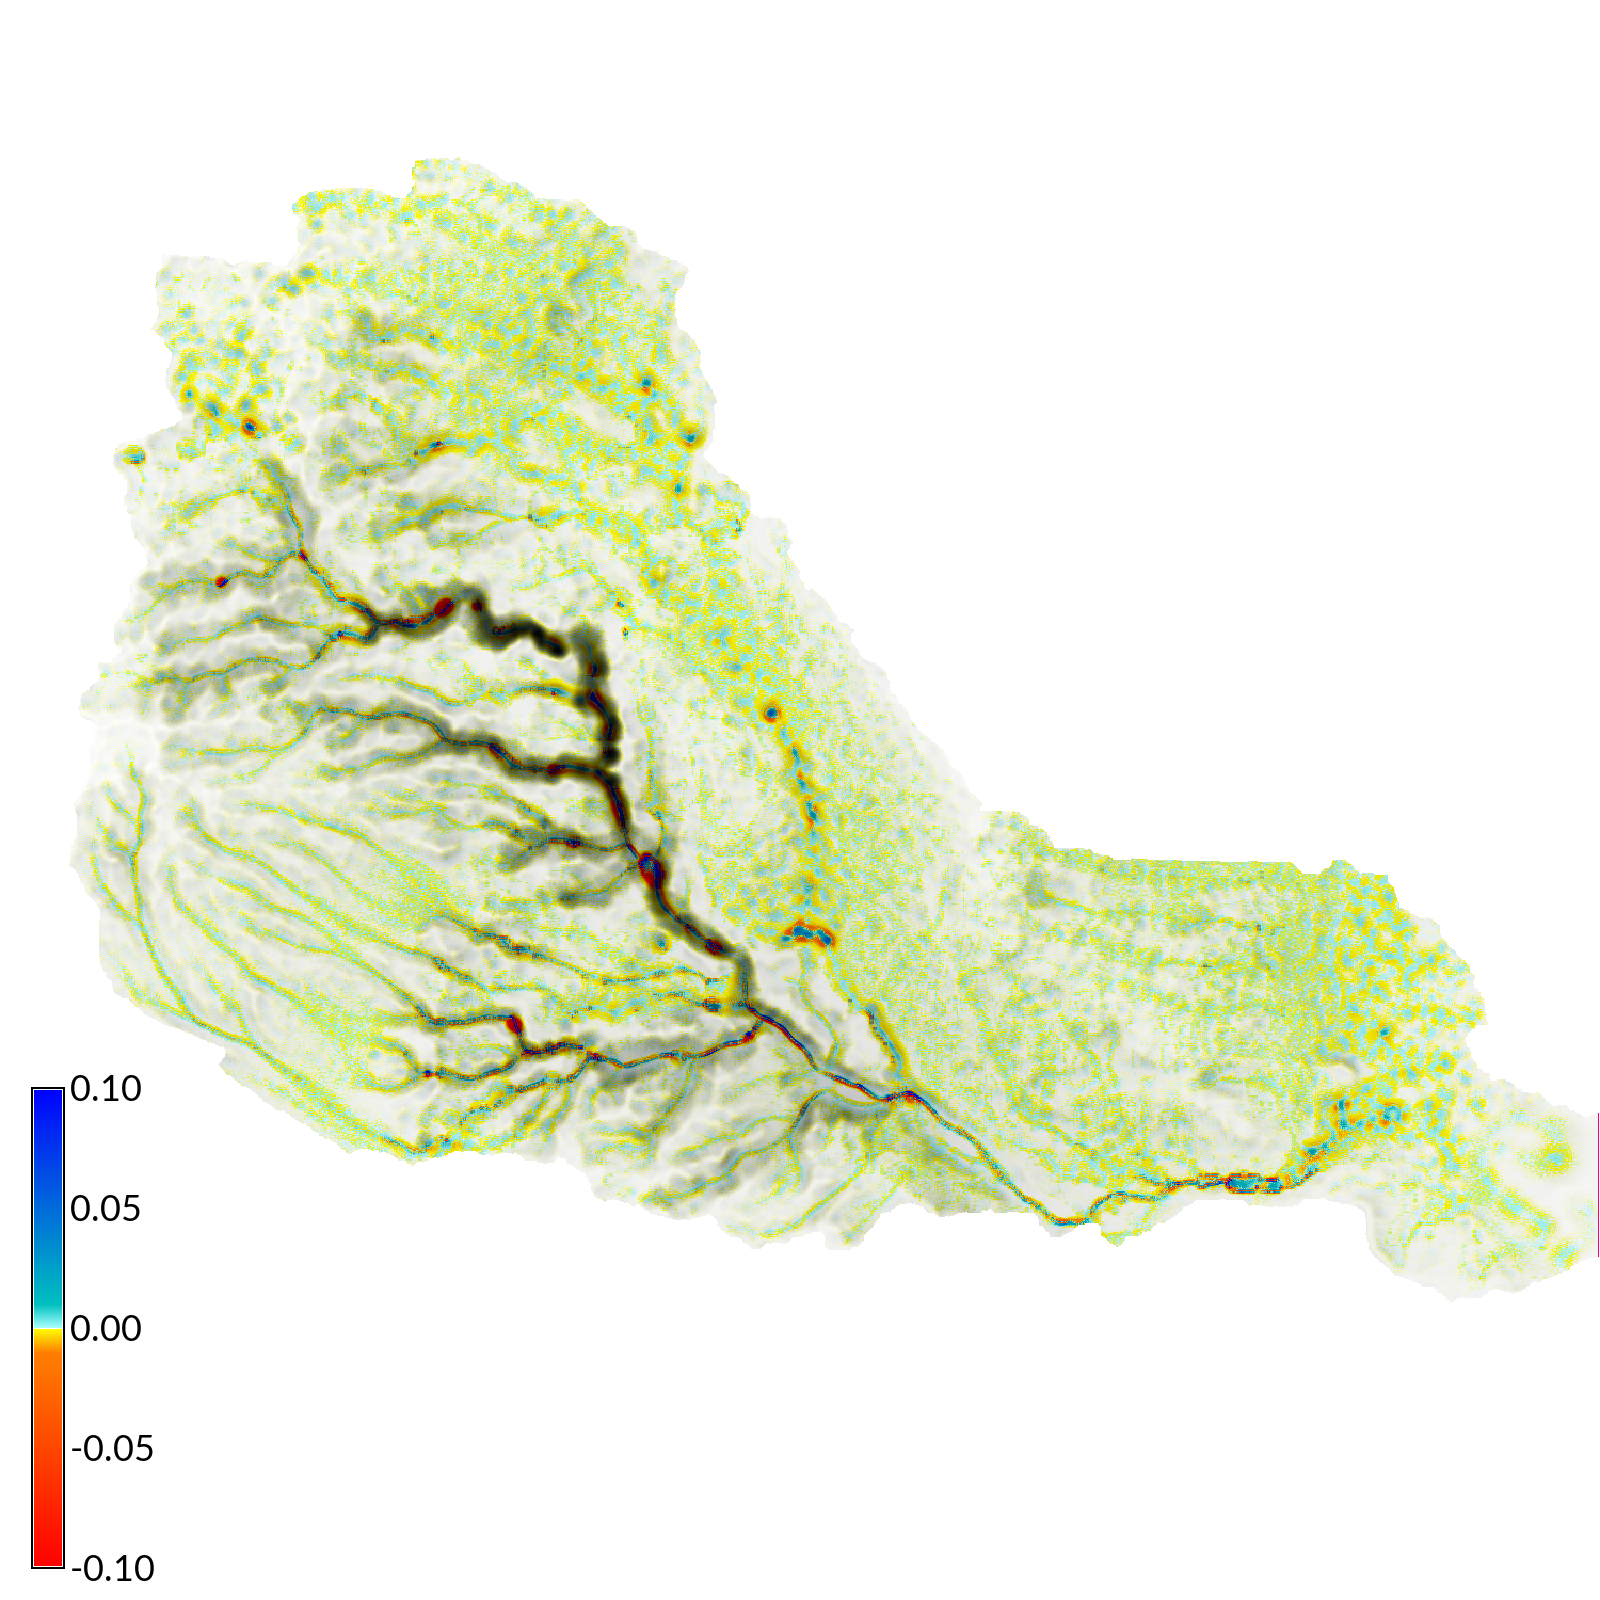
\includegraphics[width=0.75\textwidth]{../images/sample_data/erosion_deposition_2016.png}
%\caption{Erosion and deposition $(kg~m^{-2}~s^{-1})$ simulated by SIMWE}
%\label{fig:erdep}
%\end{figure}

%% source and sinks
%
%\begin{equation}\label{eq:sediment} 
%D(x,y,t) = \mathrm{source - sinks} =
%{\partial [\rho_sc(x,y,t)h(x,y,t)] \over \partial t} +
%\nabla ~ q_s(x,y,t)
%\end{equation}
%
%Sources and sinks of sediment are assumed to be proportional to
%the difference between sediment transport capacity
%and the sediment flow rate: 
%\begin{equation}\label{eq:sources_sinks} 
%d_s = \sigma [T_c  - |q_s|]
%\end{equation}

% ------------------------------------------------------------------------------

\subsubsection{Landscape evolution}

% Landscape evolution
The simulated change in elevation $\Delta z(x,y,t)$ due to water erosion and deposition
is a function of
the change in time, the net erosion-deposition rate, and the sediment mass density 
\citep{Mitasova2013}:
% landscape evolution equation
\begin{equation}
\label{eq:evolution} 
{\Delta z(x,y,t) = \Delta t ~ d_s(x,y,t) ~ \rho_s^{-1} }
\end{equation}

%{\small
%\noindent
%where: \\
%\noindent
%\hspace*{0.5em} $\Delta z =$ change in elevation $(m)$ \\
%\hspace*{0.5em} $d_s =$ net erosion-deposition $(kg ~ m^{-2} s^{-1})$ \\
%\hspace*{0.5em} $\rho_s c(x,y,t)$ = sediment mass density $(kg ~m^{-3})$\\ %[kg/m$^3$]
%\hspace*{0.5em} $\rho_s =$ sediment mass density $(kg ~m^{-3})$ \\
%}

% detachment limited landscape evolution
In a detachment limited erosion regime
the simulated change in elevation $\Delta z(x,y,t)$
is a function of
the change in time, the sediment flow rate, and the mass of water carried sediment per unit area
\citep{Mitasova2013}:
% change in elevation (m) = change in time (s) * sediment flux (kg/ms) / mass of sediment per unit area (kg/m^2)
\begin{equation}
\label{eq:flux_evolution} 
{\Delta z(x,y,t) = \Delta t ~ q_s(x,y,t) ~ \varrho_s^{-1} } 
\end{equation}
% \varrho_s(r)^{-1}
{\small
\noindent
where: \\
\noindent
%\hspace*{0.5em} $\Delta z =$ change in elevation $(m)$ \\
%\hspace*{0.5em} $q_s =$ sediment flux $(kg ~ m^{-1} s^{-1})$ \\
\hspace*{0.5em} $\varrho_s$ is the mass of sediment per unit area $(kg ~ m^{-2})$.\\
}

% ------------------------------------------------------------------------------

% gravitational diffusion
\noindent
Gravitational diffusion is then applied to the evolved topography
to simulate the settling of sediment particles. 
The simulated change in elevation $\Delta z(x,y,t) $ due to gravitational diffusion 
is a function of the change in time, the sediment mass density, 
the gravitational diffusion coefficient, and topographic divergence 
-- i.e.~the sum of the second order derivatives of elevation
\citep{thaxton2004}:
%gravitional diffusion eq.
% change in elevation (m) = elevation (m) - (change in time (s) / sediment mass density (kg/m^3) * gravitational diffusion coefficient (m^2/s) * divergence (m^-1))
\begin{equation}
\label{eq:grav_diffusion} 
{\Delta z(x,y,t) = \Delta t ~ \rho_s^{-1} ~ \varepsilon_g ~ \nabla(x,y,t)}
\end{equation}
{\small
\noindent
where: \\
\noindent
\hspace*{0.5em} $\varepsilon_g$ is the gravitational diffusion coefficient $(m^{2} s^{-1})$\\ %$(m^{-2} s^{-1})$
\hspace*{0.5em} $\nabla(x,y,t)$ is the topographic divergence $(m^{-1})$.\\
}

% -------------------------------- RUSLE --------------------------------
\subsection{Revised universal soil loss equation 3D model}
\label{rusle_model}
%RUSLE
The Revised Universal Soil Loss Equation for Complex Terrain (RUSLE3D) 
is an empirical equation for computing erosion 
in a detachment capacity limited soil erosion regime
for watersheds with complex topography \citep{Mitasova1996}. 
% USLE
It is based on 
the Universal Soil Loss Equation (USLE),
an empirical equation for estimating the average
sheet and rill soil erosion from rainfall and runoff
on agricultural fields and rangelands with simple topography 
\citep{Wischmeier1978}. 
It models erosion dominated regimes without deposition
in which sediment transport capacity is uniformly greater than detachment capacity.
As an empirical equation the predicted soil loss 
is spatially and temporally averaged. 
In USLE soil loss per unit area is determined by 
an erosivity factor $R$,
a soil erodibility factor $K$, 
a slope length factor $L$,
a slope steepness factor $S$,
a cover management factor $C$,
and a prevention measures factor $P$.
These factors are empirical constants derived 
from an extensive collection of measurements 
on 22.13 $m$ standard plots with an average slope of 9$\%$.  
%
RUSLE3D was designed to account for more complex, 3D topography 
with converging and diverging flows. 
In RUSLE3D the topographic potential for erosion at any given point 
is represented by a 3D topographic factor $LS_{3D}$,
which is a function of the upslope contributing area 
and the angle of the slope. 

In this spatially and temporally distributed model 
RUSLE3D is modified by the use of a 
event-based r-factor derived from the rainfall intensity 
at each time step.
For each time step
this model computes the parameters for RUSLE3D -- 
an event-based erosivity factor,
the slope of the topography, the flow accumulation, and
the 3D topographic factor -- and then
solves the RUSLE3D equation for sediment flow. 
The sediment flow is used to simulate landscape evolution 
in a detachment capacity limited soil erosion regime.

% RESOURCES
% https://ncsu-geoforall-lab.github.io/erosion-modeling-tutorial/erdep_theory.html
% http://www4.ncsu.edu/~hmitaso/gmslab/reports/CerlErosionTutorial/denix/denixstart.html

% ------------------------------------------------------------------------------

\subsubsection{Event-based erosivity factor}

In USLE and RUSLE the erosivity factor $R$ 
is the combination of the total energy and peak intensity of a rainfall event,
representing the interaction between the detachment of sediment particles
and the transport capacity of the flow. 
It can be calculated as the product of the 
the kinetic energy of the rainfall event $E$
and its maximum 30-minute intensity $I_{30}$
\citep{Brown1987,Renard1997}.
%
In this model, however, the erosivity factor
is derived at each time step as a function of
kinetic energy, rainfall volume, rainfall intensity, and time.
%
First rain energy is derived from rainfall intensity \citep{Brown1987}:
%
\begin{equation}
\label{eq:rain_energy}
{e_r = 0.29 ~ (1.-0.72 ~ exp(-0.05 ~ i_r))}
\end{equation}
%
{\small
\noindent
where: \\
\noindent
\hspace*{0.5em} $e_r$is unit rain energy $(MJ ~ ha^{-1} ~ mm{^-1})$\\
\hspace*{0.5em} $i_r$ is rainfall intensity $(mm ~ h^{-1})$.\\
}

\noindent
Then the event-based erosivity index $R_e$ 
is calculated as the product of 
unit rain energy, rainfall volume, rainfall intensity, and time: 
\begin{equation}
\label{eq:erosivity_index}
{R_e = e_r ~ v_r ~ i_r ~ t_r}
\end{equation}
%
{\small
\noindent
\hspace*{0.5em} $R_e$ is the event-based erosivity index $(MJ ~ mm ~ ha^{-1} ~ hr^{-1})$\\
\hspace*{0.5em} $v_r$ is rainfall volume $(mm)$ derived from ${v_r = i_r ~ t_r}$\\
\hspace*{0.5em} $t_r$ is time interval $s$\\ 
}

% ------------------------------------------------------------------------------

\subsubsection{Flow accumulation}

The upslope contributing area is determined by flow accumulation
(Fig.~\ref{fig:models}d). %(Fig.~\ref{fig:flowacc}). 
Flow accumulation is calculated using a multiple flow direction algorithm \citep{Metz2009} 
based on $A^{T}$ least cost path searches \citep{Ehlschlaeger1989}. 
The multiple flow direction algorithm 
implemented in GRASS GIS as the module 
\textit{r.watershed}\footnote{https://grass.osgeo.org/grass72/manuals/r.watershed.html}
is computationally efficient and can
navigate nested depressions and other obstacles. 

%% flow accumulation figure
%\begin{figure}[H]
%\center
%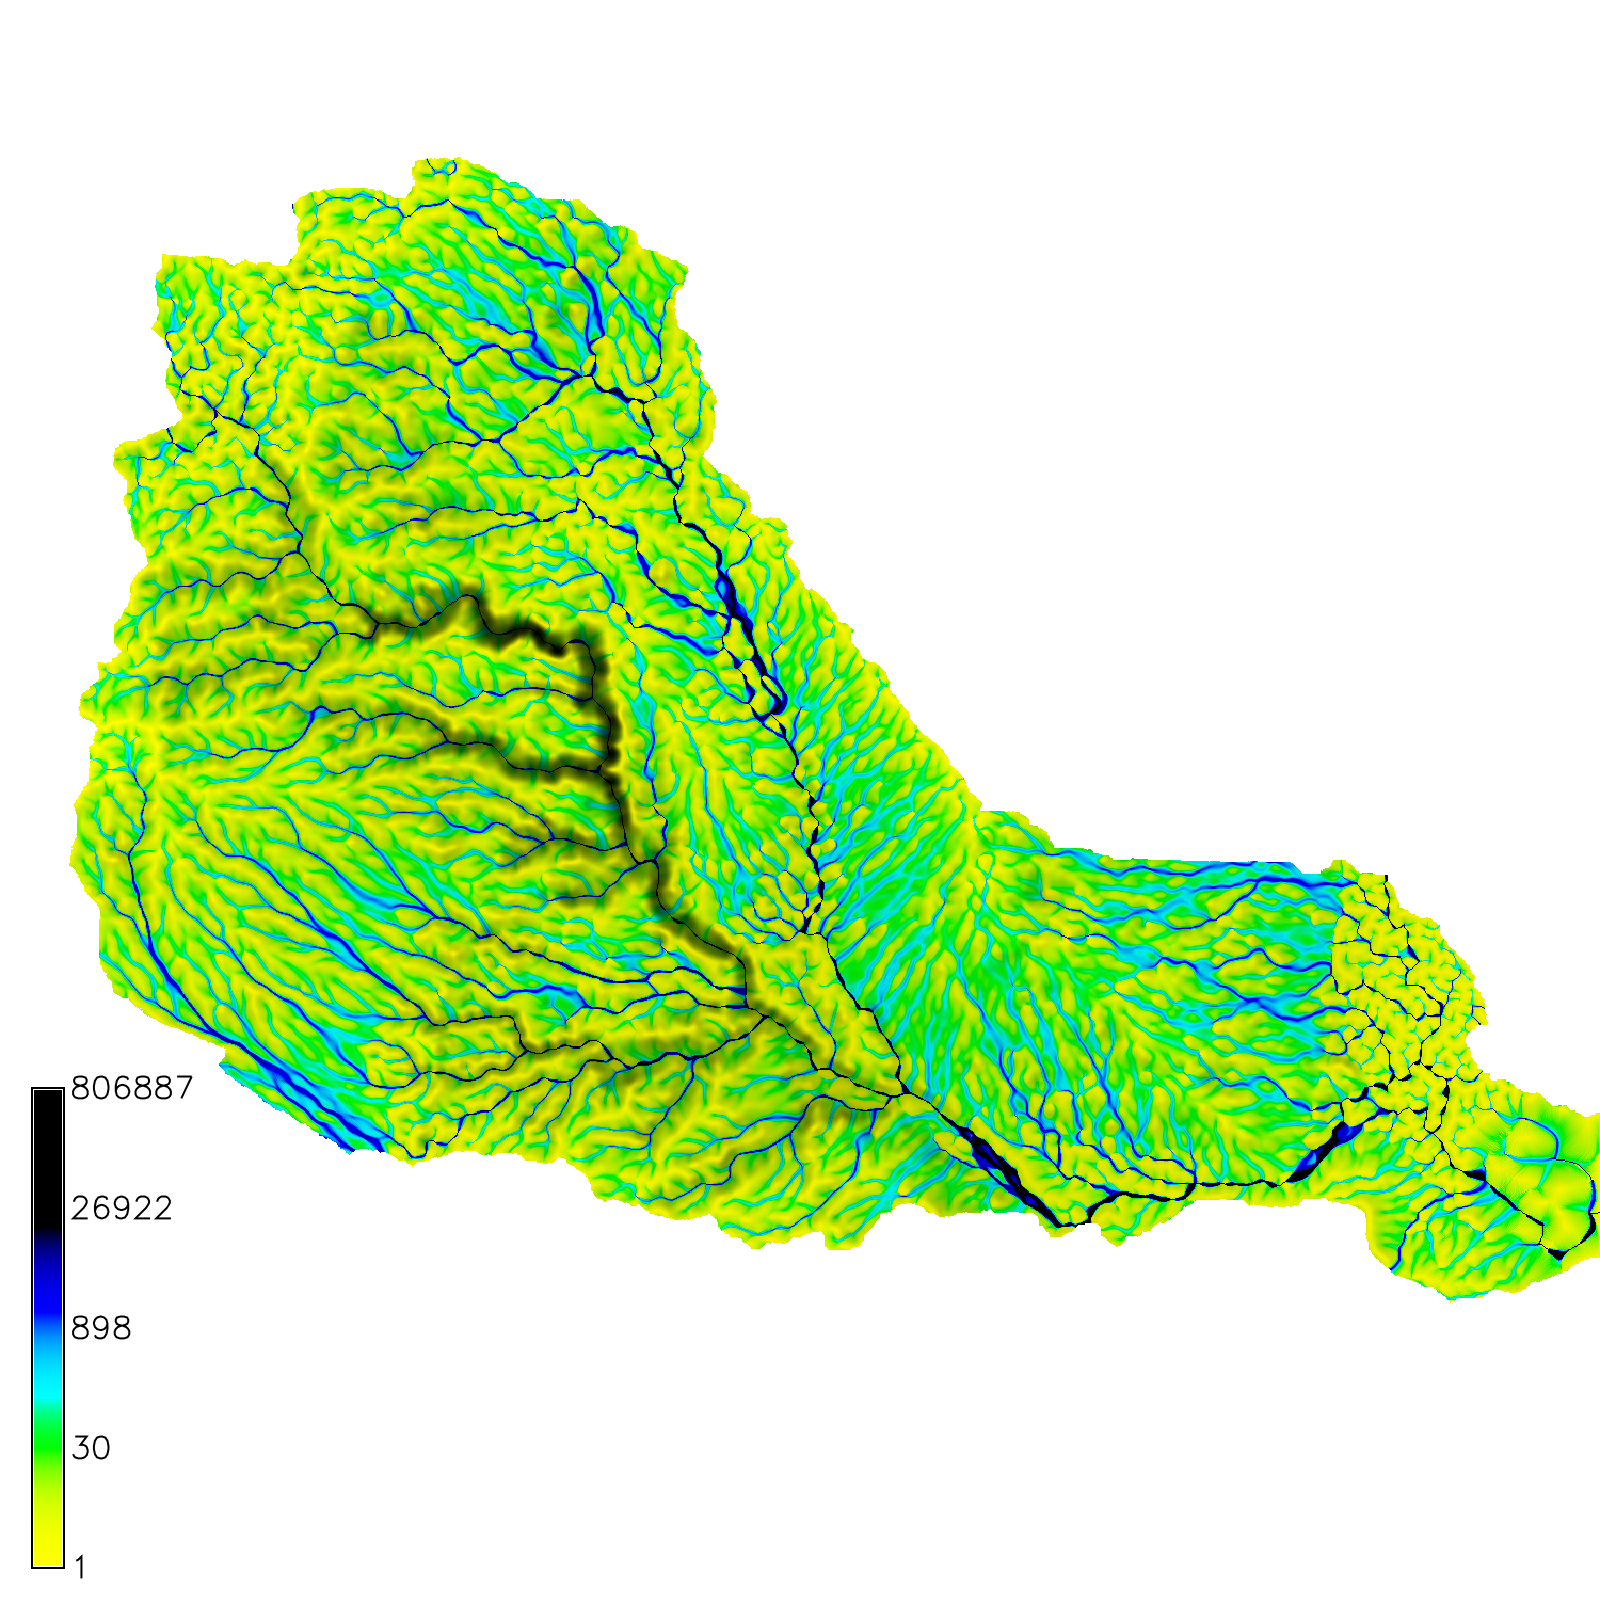
\includegraphics[width=0.75\textwidth]{../images/sample_data/flow_accumulation_2016.png}
%\caption{Flow accumulation 
%computed by multiple flow direction algorithm}
%\label{fig:flowacc}
%\end{figure}

% ------------------------------------------------------------------------------

\subsubsection{3D topographic factor}

The 3D topographic factor $LS_{3D}(x,y)$
is calculated as a function of 
the flow accumulation,
representing the upslope contributing area,
and the slope 
(Fig.~\ref{fig:models}e). %(Fig.~\ref{fig:lsfactor}). 
%
The empirical coefficients $m$ and $n$
for the upslope contributing area 
and the slope
can range from $0.2$ to $0.6$
and $1.0$ to $1.3$ respectively
with low values representing dominant sheet flow
and high values representing dominant rill flow.
%http://www4.ncsu.edu/~hmitaso/gmslab/papers/erijgis.html
%
%"with the higher values reflecting the pattern for prevailing rill erosion with more turbulent flow when erosion sharply increases with the amount of water. Lower exponent values close to m = n = 1 better reflect the pattern of compounded, long term impact of both rill and sheet erosion and averaging over a long term sequence of large and small events."
%
\begin{equation}
\label{eq:ls_factor}
{LS_{3D}(x,y) = (m+1.0) ~ (a(x,y) ~ a_0^{-1})^{m} ~ (sin(\beta) ~ \beta_0^{-1})^{n}}
\end{equation}
%
{\small
\noindent
where: \\
\noindent
\hspace*{0.5em} $LS_{3D}$ is the dimensionless topographic (length-slope) factor\\
\hspace*{0.5em} $a$ is flow accumulation $(m)$\\
\hspace*{0.5em} $a_0$ is the length of the standard USLE plot $(22.1 m)$\\
\hspace*{0.5em} $\beta$ is the slope angle $(\degree)$\\
\hspace*{0.5em} $m$ is an empirical coefficient\\
\hspace*{0.5em} $n$ is an empirical coefficient\\
\hspace*{0.5em} $\beta_0$ is the slope of the standard USLE plot $(0.09 \degree)$\\
}

%% ls factor figure
%\begin{figure}[H]
%\center
%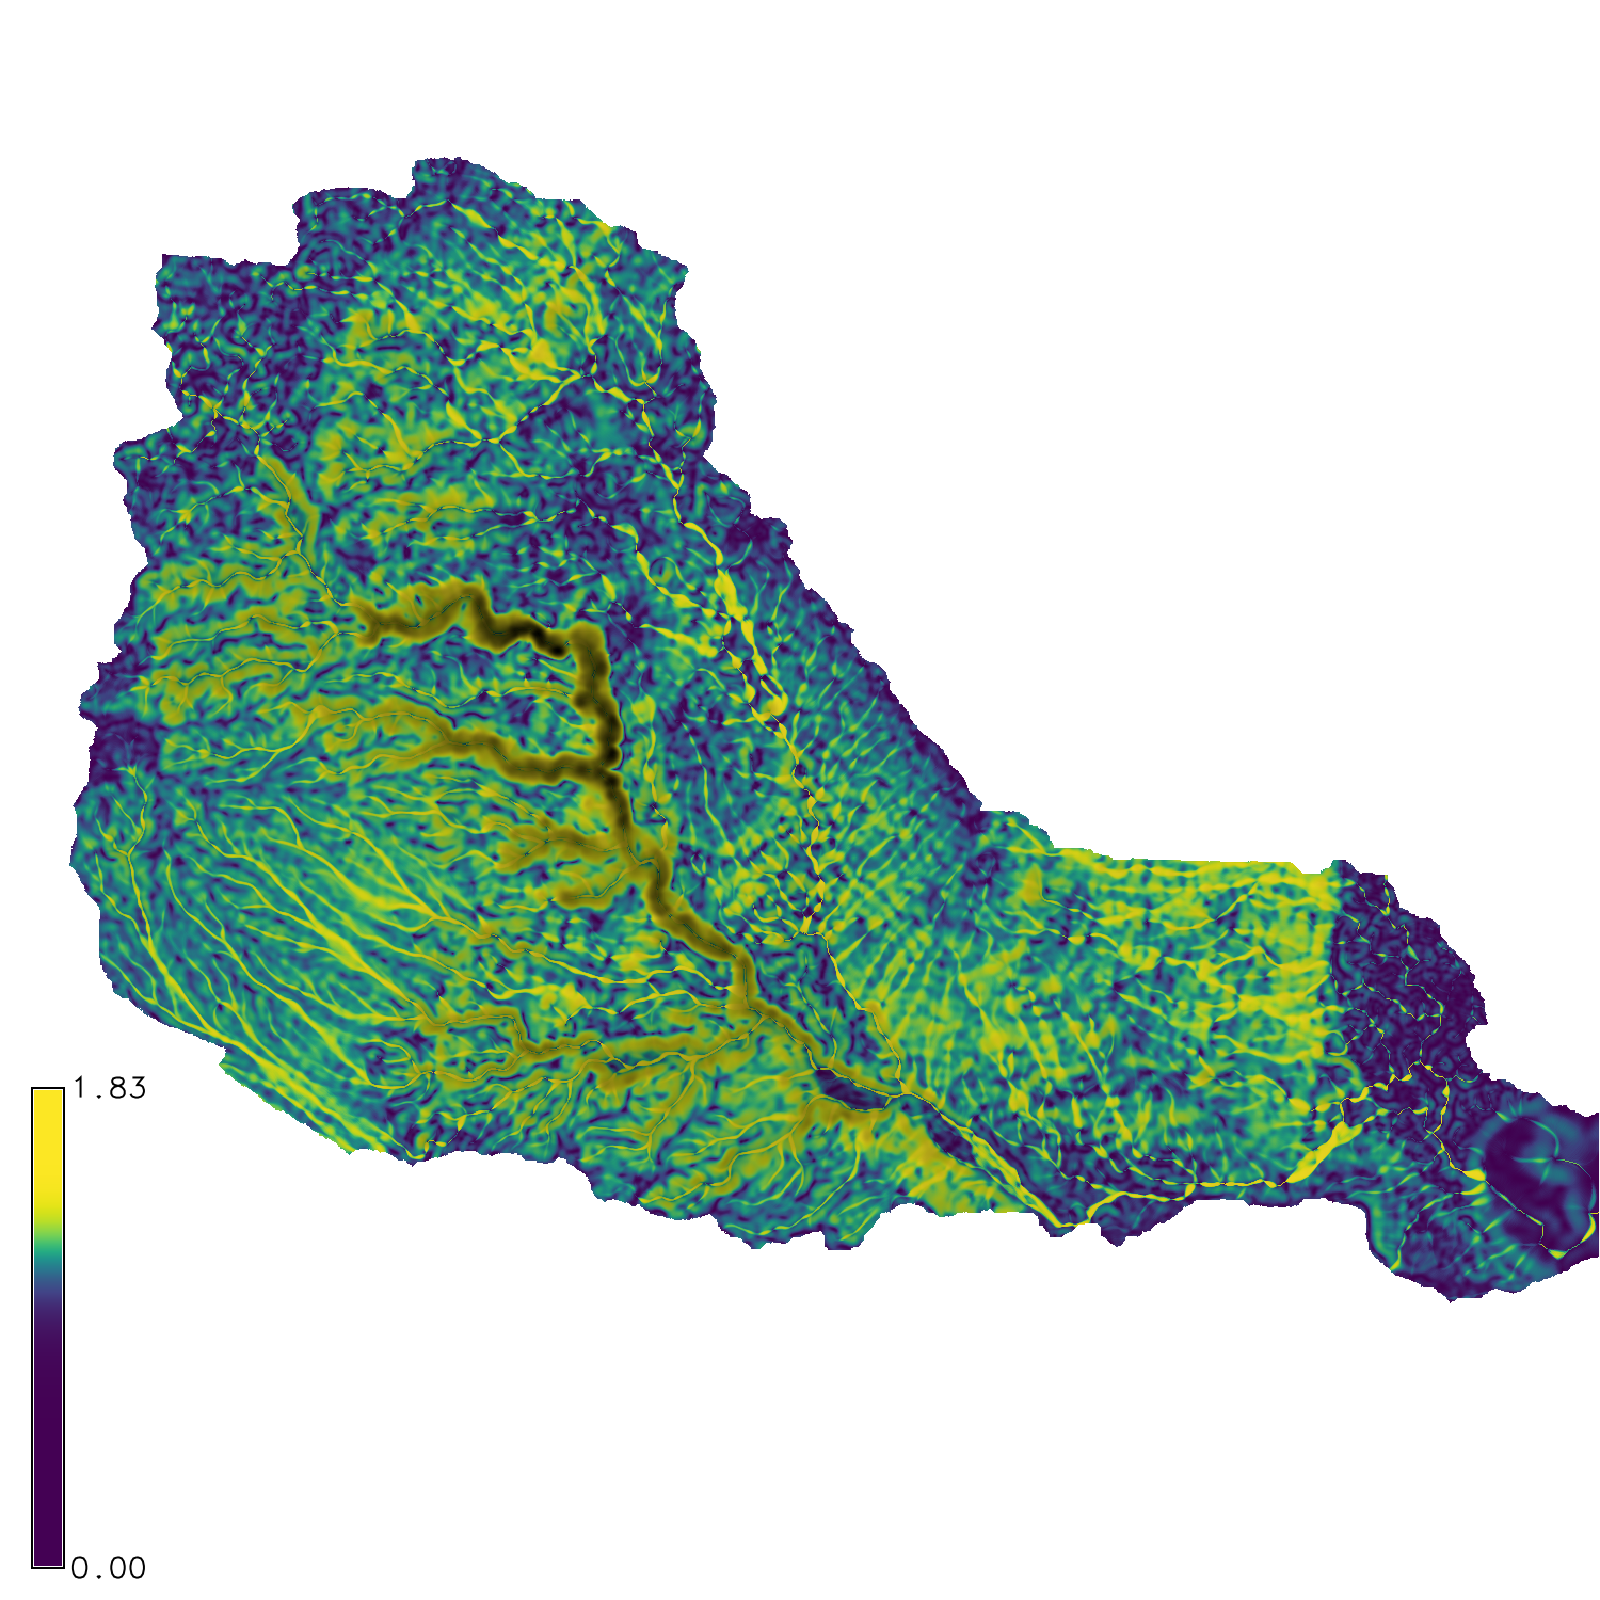
\includegraphics[width=0.75\textwidth]{../images/sample_data/ls_factor.png}
%\caption{3D topographic factor for RUSLE3D}
%\label{fig:lsfactor}
%\end{figure}

% ------------------------------------------------------------------------------

\subsubsection{Sediment flow}

The sediment flow is a function of the event-based erosivity factor, 
the soil erodibility factor, the 3D topographic factor, cover factor, and the prevention measures factor 
(Fig.~\ref{fig:models}f). %(Fig.~\ref{fig:sedflow}):
%
\begin{equation}
\label{eq:rusle}
{E = R_e ~ K ~ LS_{3D} ~ C ~ P}
\end{equation}
%
{\small
\noindent
where: \\
\noindent
\hspace*{0.5em} $E$ is soil loss $(kg ~ m^{-2} ~ min^{-1})$\\
\hspace*{0.5em} $R_e$ is the event-based erosivity factor $(MJ ~ mm ~ ha^{-1} ~ hr^{-1})$\\ %~  s{^-1}
\hspace*{0.5em} $K$ is the soil erodibility factor $(ton ~ ha ~ hr ~ ha^{-1} ~ MJ^{-1} ~ mm^{-1})$\\
\hspace*{0.5em} $LS_{3D}$ is the dimensionless topographic (length-slope) factor\\
\hspace*{0.5em} $C$ is the dimensionless land cover factor\\
\hspace*{0.5em} $P$ is the dimensionless prevention measures factor\\
}

% Landscape evolution
With RUSLE3D the simulated change in elevation $\Delta z(x,y,t)$
is derived from 
equation \ref{eq:flux_evolution}
for landscape evolution in an detachment limited soil erosion regime
and then equation \ref{eq:grav_diffusion}
for the settling of sediment particles due to gravitational diffusion.

%% sediment flow figure
%\begin{figure}[H]
%\center
%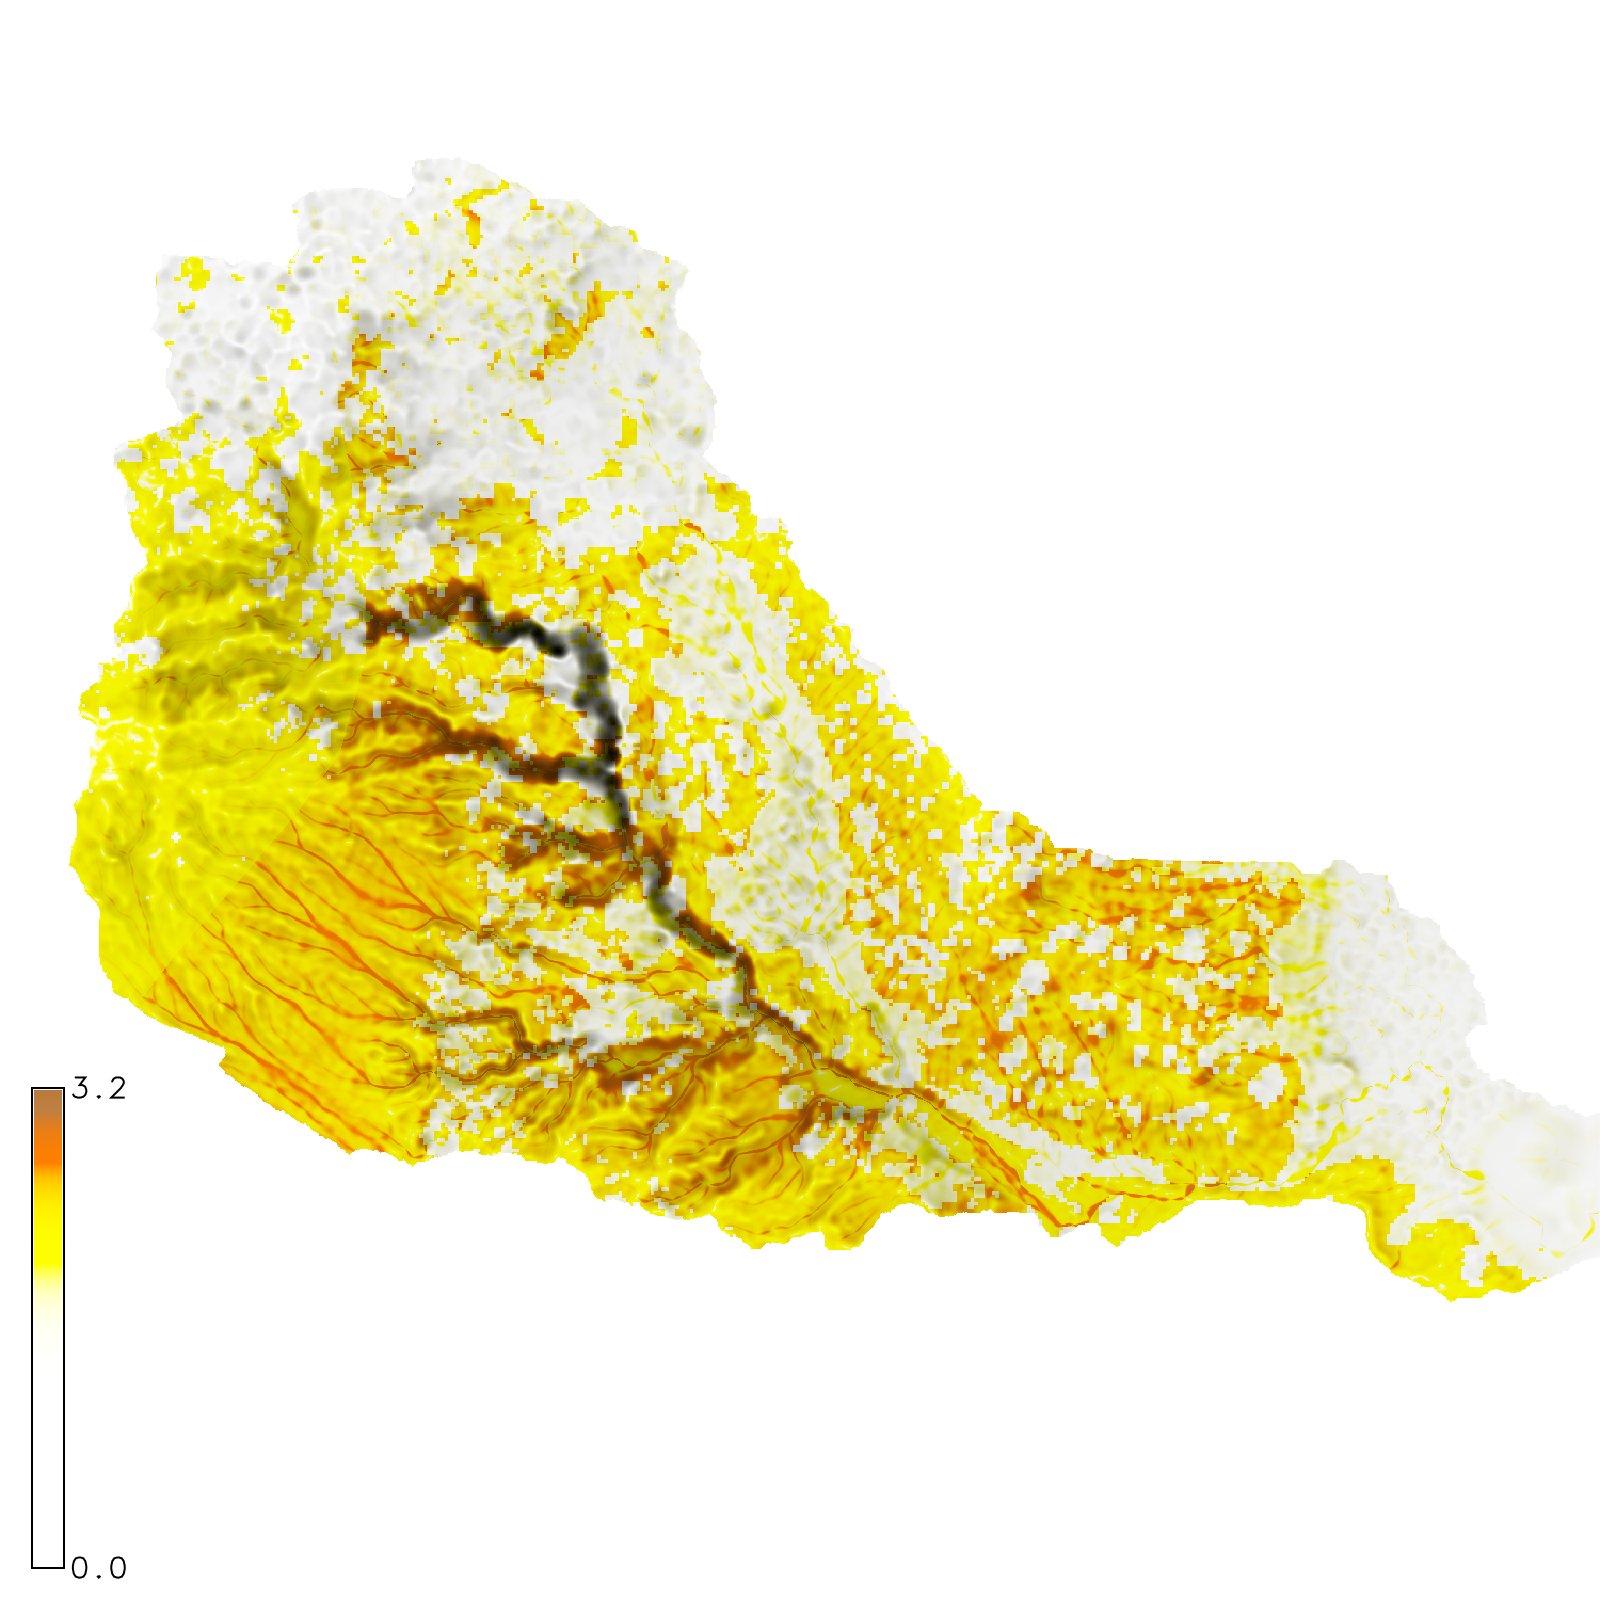
\includegraphics[width=0.75\textwidth]{../images/sample_data/sediment_flow_2016.png}
%\caption{Sediment flow modeled by RUSLE3D}
%\label{fig:sedflow}
%\end{figure}

% -------------------------------- USPED --------------------------------

\subsection{Unit streampower erosion deposition model} \label{usped_model}
The Unit Stream Power Erosion Deposition (USPED) model 
estimates net erosion-deposition as the divergence of sediment flow
in transport capacity limited soil erosion regimes.
At transport capacity 
shallow flows of water are carrying as much sediment possible 
-- more sediment is being detached 
than can be transported.
As a transport capacity limited model
USPED predicts erosion where transport capacity increases
and deposition where transport capacity decreases. 
In USPED the influence of topography on erosion and deposition
is represented by a topographic sediment transport factor,
while the influence of soil and landcover are represented by 
factors adopted from USLE and RUSLE
\citep{Mitasova1996}.

With USPED net erosion-deposition is estimated by computing
the event-based erosivity factor $R_e$ using Eq.~\ref{eq:erosivity_index},
the slope and aspect of the topography,
the flow accumulation with a multiple flow direction algorithm,
the topographic sediment transport factor,
the sediment flow at transport capacity,
and the divergence of the sediment flow. 

% Topographic sediment transport factor
For USPED
the 3D topographic factor (Eq.~\ref{eq:ls_factor} for RUSLE3D 
is adapted to represent the topographic sediment transport factor $LST$ --
the topographic component 
of overland flow at sediment transport capacity:
%
\begin{equation}
\label{eq:lst_factor}
{LST = U^{m} ~ (\sin \beta)^{n}}
\end{equation}
%
{\small
\noindent
where: \\
\noindent
\hspace*{0.5em} $LST$ is the topographic sediment transport factor\\
\hspace*{0.5em} $U$ is the flow accumulation $(m)$\\
\hspace*{0.5em} $\beta$ is the angle of the slope $(\degree)$\\
\hspace*{0.5em} $m$ is an empirical coefficient\\
\hspace*{0.5em} $n$ is an empirical coefficient.\\
}

% Sediment flow at transport capacity
The sediment flow at transport capacity is a function of 
the event-based rainfall factor, the soil erodibility factor, 
the topographic component of overland flow,
tje landcover factor, and the prevention measures factor:
%
\begin{equation}
\label{eq:usped}
{T = R_e ~ K ~ C ~ P ~ LST}
\end{equation}
{\small
\noindent
where: \\
\noindent
\hspace*{0.5em} $T$ is sediment flow at transport capacity $(kg ~ m^{-1} ~ s^{-1})$\\ 
\hspace*{0.5em} $R_e$ is the event-based rainfall factor $(MJ ~ mm ~ ha^{-1} ~ hr^{-1})$\\
\hspace*{0.5em} $K$ is the soil erodibility factor $(ton ~ ha ~ hr ~ ha^{-1} ~ MJ^{-1} ~ mm^{-1})$\\ % check units
\hspace*{0.5em} $C$ is the dimensionless land cover factor\\
\hspace*{0.5em} $P$ is the dimensionless prevention measures factor.\\
}

%Erosion-deposition at transport capacity
Net erosion-deposition at transport capacity is estimated as the divergence of sediment flow: 
%D = ∇ · (T s0) = ∂(T cos α)/∂x + ∂(T sin α)/∂y
\begin{equation}\label{eq:usped_erdep} 
d_s(x,y,t) = 
{\partial (T ~ \cos \alpha) \over \partial x} +
{\partial (T ~ \sin \alpha) \over \partial y}
\end{equation}
{\small
\noindent
where: \\
\hspace*{0.5em} $d_s(x,y,t)$ is net erosion-deposition $(kg ~ m^{-2} s^{-1})$\\
\hspace*{0.5em} $\alpha$ is the aspect of the topography ($\degree$).\\
}

%Landscape evolution
With USPED the simulated change in elevation $\Delta z(x,y,t)$
is derived from equation \ref{eq:evolution} for landscape evolution
and then equation \ref{eq:grav_diffusion}
for the settling of sediment particles due to gravitational diffusion.

% -------------------------------- CASE STUDIES --------------------------------

\begin{figure}[H]
\centering
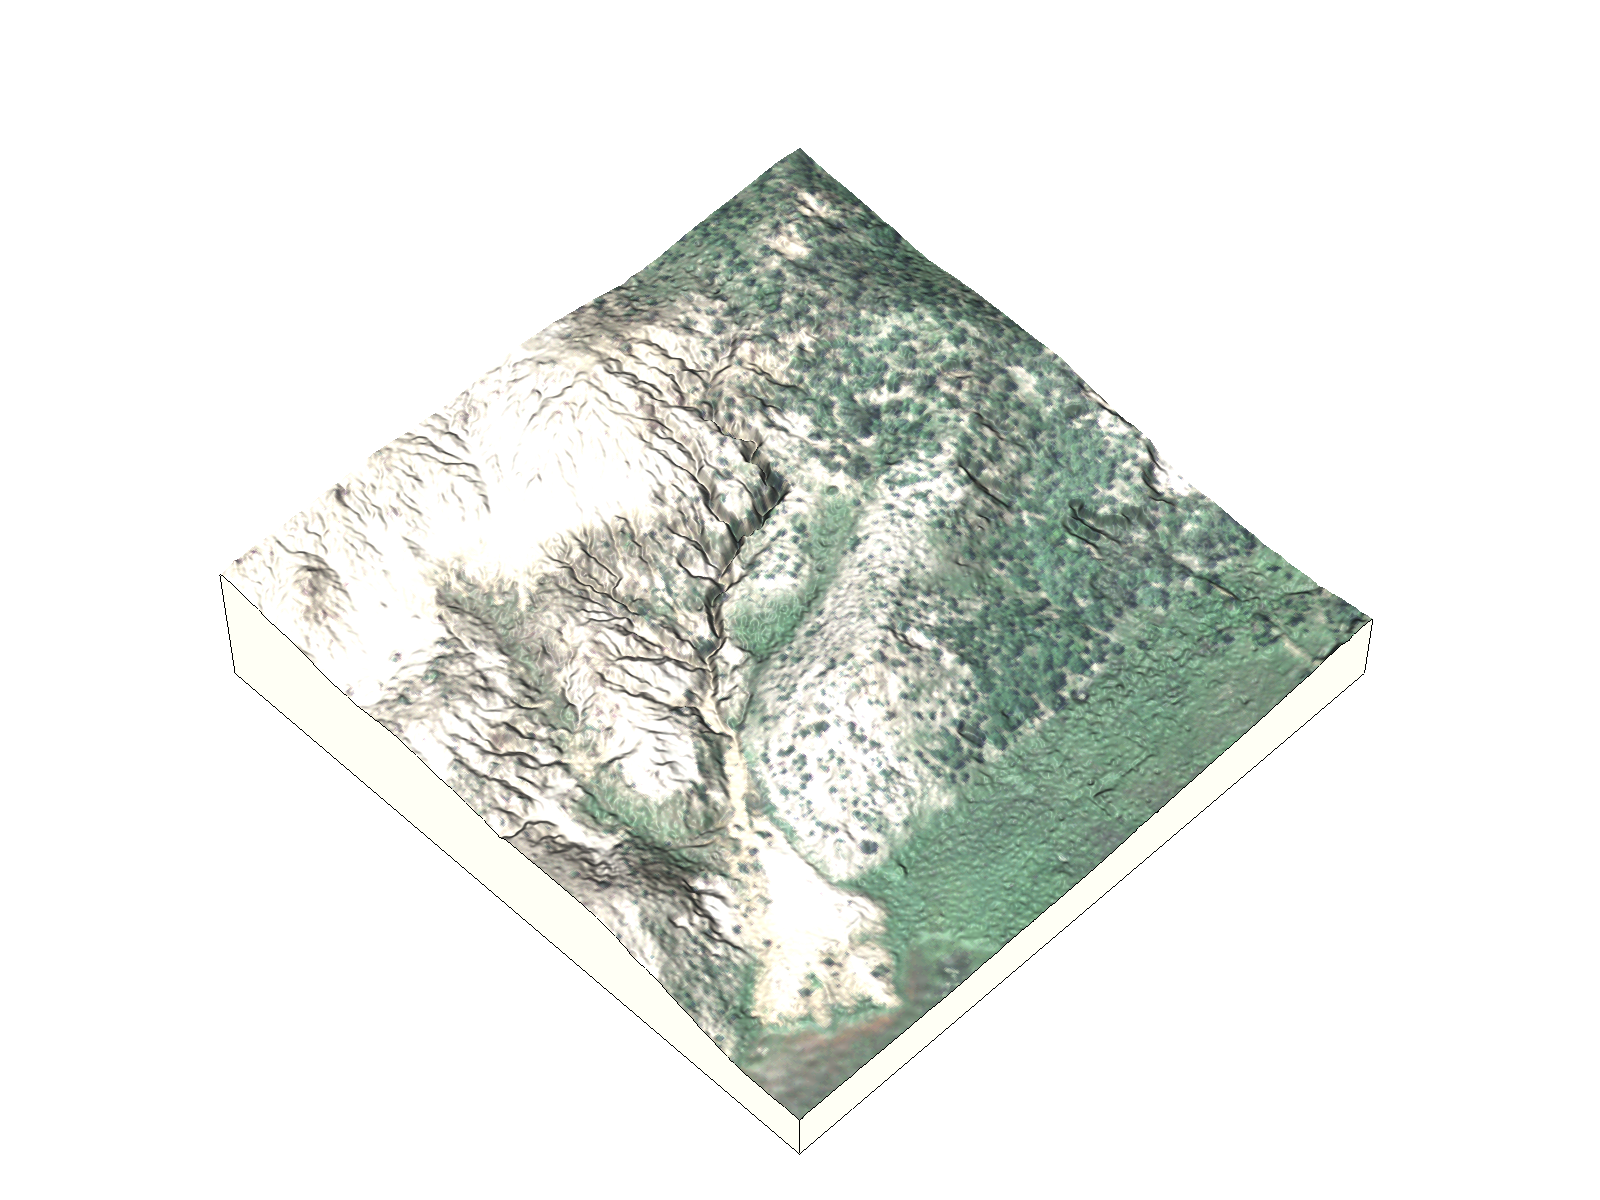
\includegraphics[width=0.75\textwidth]{../images/sample_data_3d/naip_2014.png}
\caption{Study landscape, Patterson Branch Creek, Fort Bragg, NC, USA}
\label{fig:3d}
\end{figure}

\section{Case studies} 

%\subsection{Fort Bragg}
%...
% map of fort bragg with shaded landcover and watersheds

% map of fort bragg with shaded relief and watersheds

% map of fort bragg erosion with rusle3d

% map of difference for fort bragg

\subsection{Patterson Branch Creek}
%
To test the effectiveness of r.sim.terrain's models 
we compared the simulated evolution
of a highly eroded subwatershed of 
Patterson Branch Creek on Fort Bragg, North Carolina
against a timeseries of lidar surveys.
The models -- SIMWE, RUSLE3D, and USPED --
were tested in steady state and dynamic modes
for constant rainfall, design storms, and recorded rainfall.

% --------- STUDY AREA ---------
Fort Bragg, a military installation 
in the Sandhills region of North Carolina % sq meters? 650 km2
with a Longleaf Pine and Wiregrass Ecosystem \citep{Sorrie2006},
has extensive areas of bare, erodible soils
on impact areas, firing ranges, landing zones, and dropzones. 
%
The study landscape
-- a subwatershed of Patterson Branch Creek 
% how many square meters is the subwatershed?
in the Coleman Impact Area --
is pitted with impact craters from artillery and mortar shells
and has an active, approximately $2~m$ deep gully. 
%
It is a Pine-Scrub Oak Sandhill community
composed primarily of Longleaf Pine -- Pinus palustris --
and Wiregrass -- Aristida stricta --
on Blaney and Gilead loamy sands 
\citep{Sorrie2004}. 
%
Throughout the Coleman Impact Area
the frequent fires ignited by live munitions
drive the ecological disturbance regime
of this fire adapted ecosystem.
%
In 2016 the  $450~m^{2}$ study site was
43.24\% bare ground with predominately loamy sands,
39.54\% covered by the Wiregrass community, and
17.22\% forested with the Longleaf Pine community 
(Figure~\ref{fig:study_area}c). 
%
We hypothesize that the elimination of forest cover
in the impact zone
triggered extensive channelized overland flow,
gully formation, and sediment transport into the creek. 

% --------- DATA ---------
We generated a timeseries of 
digital elevations models and landcover maps 
of the study landscape
from lidar pointclouds and orthophotography
(Figure~\ref{fig:study_area}a-c). 
%
The digital elevations models for 2004, 2012, and 2016
were interpolated at $0.3~m$ resolution
using the regularized spline with tension function \citep{Mitasova1993,Mitasova2005}
\footnote{https://grass.osgeo.org/grass74/manuals/v.surf.rst.html}
from %$1~m$ resolution 
airborne lidar surveys 
collected by the NC Floodplain Mapping program and Fort Bragg. 
%
Unsupervised image classification 
\footnote{https://grass.osgeo.org/grass74/manuals/i.maxlik.html}
was used to identify clusters of spectral reflectance
\footnote{https://grass.osgeo.org/grass74/manuals/i.cluster.html}
in a timeseries of 1 meter resolution orthoimagery 
collected by the National Agriculture Imagery Program.
%
The landcover maps were derived by fusing the
classified lidar point clouds with the classified orthoimagery.
%
Spatially variable soil erosion factors 
-- k-factor, c-factor, mannings, and runoff rates --
were derived from the landcover and soil maps.
%
The dataset for this study is hosted at 
\url{https://github.com/baharmon/landscape\_evolution_dataset}
under the ODC Open Database License (ODbL).
%
The data is derived from publicly available data from
the US Army, USGS, USDA, Wake County GIS, NC Floodplain
Mapping Program, and the NC State Climate Office.

% --------- MORPHOLGY ---------
We used the geomorphons method 
\footnote{https://grass.osgeo.org/grass74/manuals/r.geomorphon.html}
of automated landform classification
based on the openness of terrain \citep{Jasiewicz2013}
and the difference between the digital elevation models 
to analyze the changing morphology of the study area
(Figure~\ref{fig:study_area}d-f). 
%
The $2~m$ deep gully -- 
its channels classified as valleys and 
its scour pits as depressions by geomorphons -- 
has multiple mature branches
and ends with a depositional fan.
%
The gully has also developed 
depositional ridges beside the channels.
Deep scour pits have developed 
where branches join the main channel 
and where the main channel has sharp bends.
%
A new branch has begun to form 
in a knickzone classified as a mix of valleys and hollows
on a grassy swale on the northeast side of the gully.
Between 2012 and 2016 a depositional ridge
has developed at the foot of this nascent branch
where it would meet the main channel. 
%
The difference in elevation between 2012 and 2016
(Figure~\ref{fig:study_area}d)
shows a deepening of the main channel 
by approximately $0.2~m$ 
and the scours pits
by approximately $1~m$,
while depositional ridges have formed and grown up to
approximately $1~m$ or more.
% add figure with labeled features

% study area figure
\begin{figure}[H]
\center
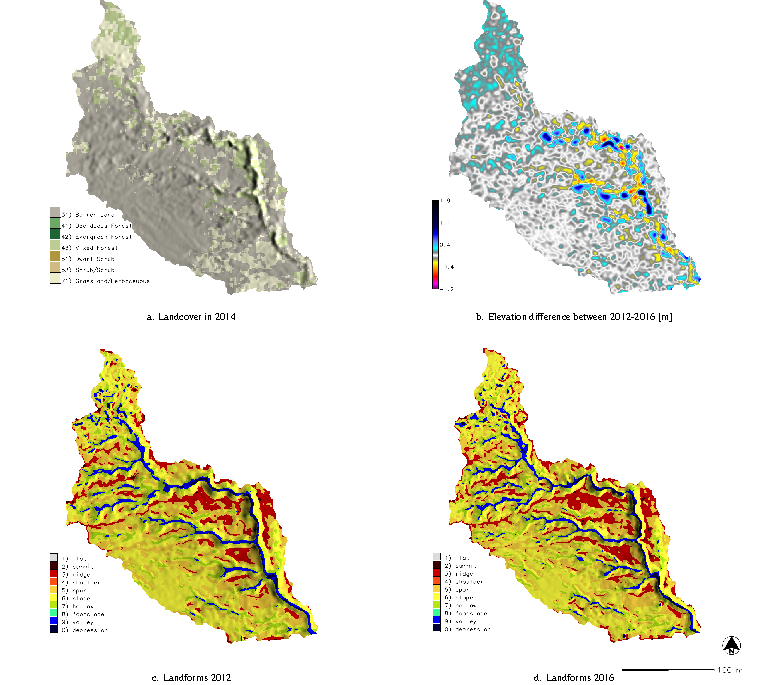
\includegraphics[width=\textwidth,height=0.95\textheight,keepaspectratio]{figures/study_area.pdf}
\caption{Study Landscape, Patterson Branch Creek, Fort Bragg, NC, USA}
\label{fig:study_area}
\end{figure}


% --------- SIMULATIONS ---------
\subsubsection{Simulations}
%
We ran a sequence of simulations 
for the Patterson Branch Creek subwatershed study area
to test dynamic and steady state flow regimes
in the SIMWE, RUSLE3D, and USPED models
(Table~\ref{table:simulations}).
%
We used RUSLE3D to simulate $120~min$ events
with rainfall intensities of $50~mm~hr^{-1}$
for detachment capacity limited soil erosion regimes
for both dynamic and steady state flow regimes
using RUSLE3D
(Figure~\ref{fig:simulations}a-c).
% 
We used USPED to simulate $120~min$ events
with rainfall intensities of $50~mm~hr^{-1}$
for transport capacity limited soil erosion regimes
for both dynamic and steady state flow regimes
(Figure~\ref{fig:simulations}d-f).
%
We used SIMWE to simulate $120~min$ events 
with rainfall intensities of $50~mm~hr^{-1}$
for erosion-deposition 
and detachment limited soil erosion regimes 
in steady state flow regimes
(Figure~\ref{fig:simwe_simulations}).
%
In all of the simulations 
we used a sink filling algorithm 
-- an optional parameter in r.sim.terrain --  
to reduce the effects of positive feedback loops
that cause the over-development of scour pits. 

% scripts
The simulations were automated and run in parallel
using Python scripts that are available in the 
\href{https://github.com/baharmon/landscape_evolution}{software repository}.
% reproducibility
The simulations can be reproduced using these scripts
and the study area dataset 
by following the instructions 
in the Open Science Framework repository 
at \url{https://osf.io/tf6yb/}.
% benchmarks
The simulations were run 
in GRASS GIS 7.4 
on a desktop computer 
with 64-bit Ubuntu 16.04.4 LTS,
8 x 4.20 GHz Intel Core i7 7700K CPUs,
and 32 GB RAM. 
% runtime
Dynamic simulations of RUSLE3D and USPED each took
$3~min~14~s$ to run on a single thread, 
while steady state simulations for SIMWE each took 
$84~min~13~s$ running on 6 threads
(Table~\ref{table:simulations}).
% multithreading
Simulations using SIMWE 
are far more computationally intensive
and thus take much more time to run
than RULSE3D or USPED, 
but support multi-threading 
when compiled with OpenMP. 

% results

% rusle works great and fast!
% overly incised channel compared to simwe flux
% detachment limited vs. detachment limited models

% flux works well, causes 


% --------- SIMULATION TABLE ---------

% table of simulations
\begin{table*}
\small
\caption{Landscape evolution simulations}
\begin{tabu} to \textwidth {XXXXXllllllX}
\toprule
Dynamics & Model & Intensity & Duration & Interval & $D_c$ & $T_c$ & m & n & $\rho_s$ & Threads & Runtime\\
\midrule
Dynamic & RUSLE3D & $50~mm~hr^{-1}$ & $120~min$ & $3~min$ &  &  & 0.4 & 1.3 & & & $3~min~14~s$\\
Dynamic & USPED & $50~mm~hr^{-1}$ & $120~min$ & $3~min$ &  &  & 1.5 & 1.2 & 1.6 & & $3~min~14~s$\\
Steady state & RUSLE3D & $75~mm~hr^{-1}$ & $120~min$ & $120~min$ &  &  & 0.4 & 1.3 & \\
Steady state & USPED & $50~mm~hr^{-1}$ & $120~min$ & $120~min$ &  &  & 1.5 & 1.2 & 1.6\\
Steady state & SIMWE & $50~mm~hr^{-1}$ & $120~min$ & $120~min$ & 0.001 & & & & 1.6 & 6 & $84~min~13~s$\\
Steady state & SIMWE & $25~mm~hr^{-1}$ & $120~min$ & $120~min$ & 0.0001 & 0.01 & & & 1.6 & 6 & $84~min~13~s$\\
\bottomrule
\\
\end{tabu}
\label{table:simulations} 
\end{table*}

% add runtimes for steady state rusle3d and usped

% --------- SIMULATION FIGURES ---------

% dynamic vs steady state figure
\begin{figure}[H]
\center
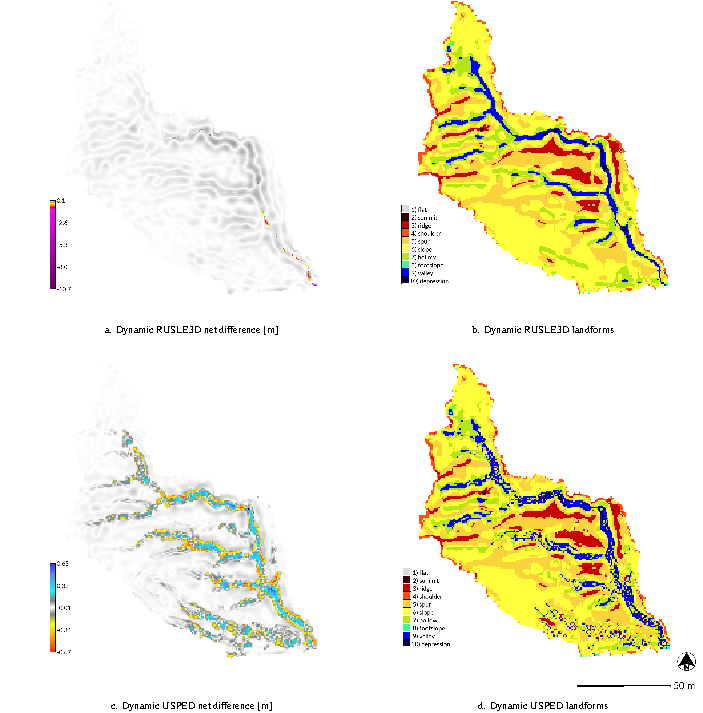
\includegraphics[width=\textwidth,height=0.925\textheight,keepaspectratio]{figures/simulations.pdf}
\caption{Dynamic and steady state RUSLE3D and USPED simulations
for a $120~min$ event} % with a rainfall intensity of $50~mm~hr^{-1}$}
\label{fig:simulations}
\end{figure}

% steady state simwe figure
\begin{figure}[H]
\center
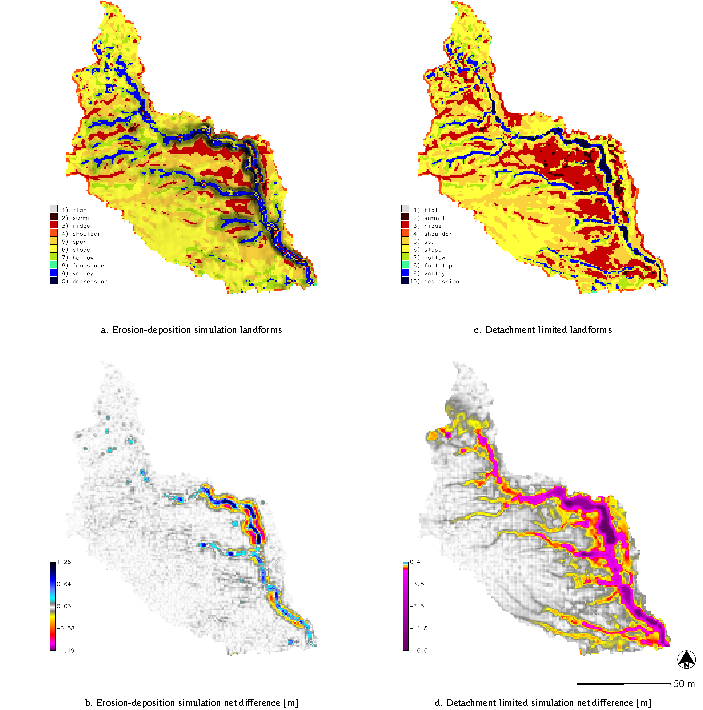
\includegraphics[width=\textwidth,height=0.95\textheight,keepaspectratio]{figures/simwe.pdf}
\caption{Steady state SIMWE simulations
for a $120~min$ event with a rainfall intensity of $50~mm~hr^{-1}$}
\label{fig:simwe_simulations}
\end{figure}

% rerun RUSLE3D and USPED with 50 mm/hr
% add legends and watershed to 3D renderings
% add mask to 2D renderings
% check landform params
% check rusle 3d sedflow in min or sec


% -------------------- DISCUSSION ---------------------------------
%\section{Discussion}

% -------------------- CONCLUSIONS ---------------------------------

\conclusions %[modified heading if necessary]
...

% --------------------CODE AND DATA------------------------

\codedataavailability{
% Code
The Python source code for the landscape evolution model 
is available on GitHub at 
\url{https://github.com/baharmon/landscape_evolution}
under the GNU General Public License version 2. 
This repository also includes Python scripts 
for running and reproducing the simulations in this paper. 
% Docker
%
% Data
The geospatial dataset for the study area is available on GitHub at
\url{https://github.com/baharmon/landscape_evolution_dataset}
under the 
\href{https://opendatacommons.org/licenses/odbl/}{Open Database License}. 
% OSF
The source code, scripts, data, and results are available 
on the Open Science Framework at 
\url{https://osf.io/tf6yb/}.
} 

% ----------------------------------------------------------------------------

\noappendix %use this to mark the end of the appendix section

% ----------------------------------------------------------------------------

\authorcontribution{
Brendan Harmon developed 
the models, code, data, case studies, and text.
Helena Mitasova contributed to the development 
of the models and case studies. 
Anna Petrasova and Vaclav Petras
contributed to the development of the code.
}

\competinginterests{The authors declare that they have no conflict of interest.} 

%\begin{acknowledgements}
%GRASS Development Community
%\end{acknowledgements}

% ---------------------REFERENCES---------------------------
\bibliographystyle{copernicus}
\bibliography{landscape_evolution.bib}

% -------------------- TEMPLATE ------------------

%\appendix
%\section{} %Appendix A
%\subsection{} %Appendix A1, A2, etc.

%% Regarding figures and tables in appendices, the following two options are possible depending on your general handling of figures and tables in the manuscript environment:

%% Option 1: If you sorted all figures and tables into the sections of the text, please also sort the appendix figures and appendix tables into the respective appendix sections.
%% They will be correctly named automatically.

%\appendixfigures  %% needs to be added in front of appendix figures
%
%\appendixtables   %% needs to be added in front of appendix tables

%% Please add \clearpage between each table and/or figure. Further guidelines on figures and tables can be found below.

%%% ONE-COLUMN TABLE
%
%%t
%\begin{table}[t]
%\caption{TEXT}
%\begin{tabular}{column = lcr}
%\tophline
%
%\middlehline
%
%\bottomhline
%\end{tabular}
%\belowtable{} % Table Footnotes
%\end{table}

%%% MATHEMATICAL EXPRESSIONS
%
%%% All papers typeset by Copernicus Publications follow the math typesetting regulations
%%% given by the IUPAC Green Book (IUPAC: Quantities, Units and Symbols in Physical Chemistry,
%%% 2nd Edn., Blackwell Science, available at: http://old.iupac.org/publications/books/gbook/green_book_2ed.pdf, 1993).
%%%
%%% Physical quantities/variables are typeset in italic font (t for time, T for Temperature)
%%% Indices which are not defined are typeset in italic font (x, y, z, a, b, c)
%%% Items/objects which are defined are typeset in roman font (Car A, Car B)
%%% Descriptions/specifications which are defined by itself are typeset in roman font (abs, rel, ref, tot, net, ice)
%%% Abbreviations from 2 letters are typeset in roman font (RH, LAI)
%%% Vectors are identified in bold italic font using \vec{x}
%%% Matrices are identified in bold roman font
%%% Multiplication signs are typeset using the LaTeX commands \times (for vector products, grids, and exponential notations) or \cdot
%%% The character * should not be applied as mutliplication sign

%%% PHYSICAL UNITS
%%% Please use \unit{} and apply the exponential notation

\end{document}
